\chapter{Evaluation}
\label{chap:evaluation}

The presented map-merging algorithm (Chapter~\ref{chap:mergingalgorithm}) has been evaluated on a number of demanding robotics datasets. The datasets include data captured by small aerial vehicles (Sections~\ref{sec:euroc-dataset}, \ref{sec:aau-dataset}) as well as ground-based robots. The datasets include both widely used benchmark datasets in robotics research as well as data recorded by the author.

Sensors used include stereo rig cameras and active \gls{RGB-D} cameras, which are popular visual sensors in the mobile robotics. This variety of sensors and robots covers many typical multi-robot deployments. All datasets have been captured under real-world conditions, none of them uses simulated data.

The evaluation focuses on properties of the presented pair-wise transformation estimation algorithm for point clouds (Section~\ref{sec:estimate-pair-wise}), which is the core algorithm of the implemented map-merging \gls{ROS} node (Section~\ref{sec:ros-package}). The accuracy of the estimation algorithm is critical for the overall map-merging process.

\section{The EuRoC micro aerial vehicle dataset collection}
\label{sec:euroc-dataset}

The publicly available datasets introduced by~\citet{Burri2016} was collected onboard a micro aerial vehicle (Figure~\ref{fig:euroc_platform}) equipped with a stereo camera rig and an \gls{IMU}. Calibration data for the cameras and ground-truth data are provided with the dataset. This dataset has been used extensively by researches for evaluation of the visual \gls{SLAM} algorithms and visual odometry approaches.

\begin{figure}
    \centering
    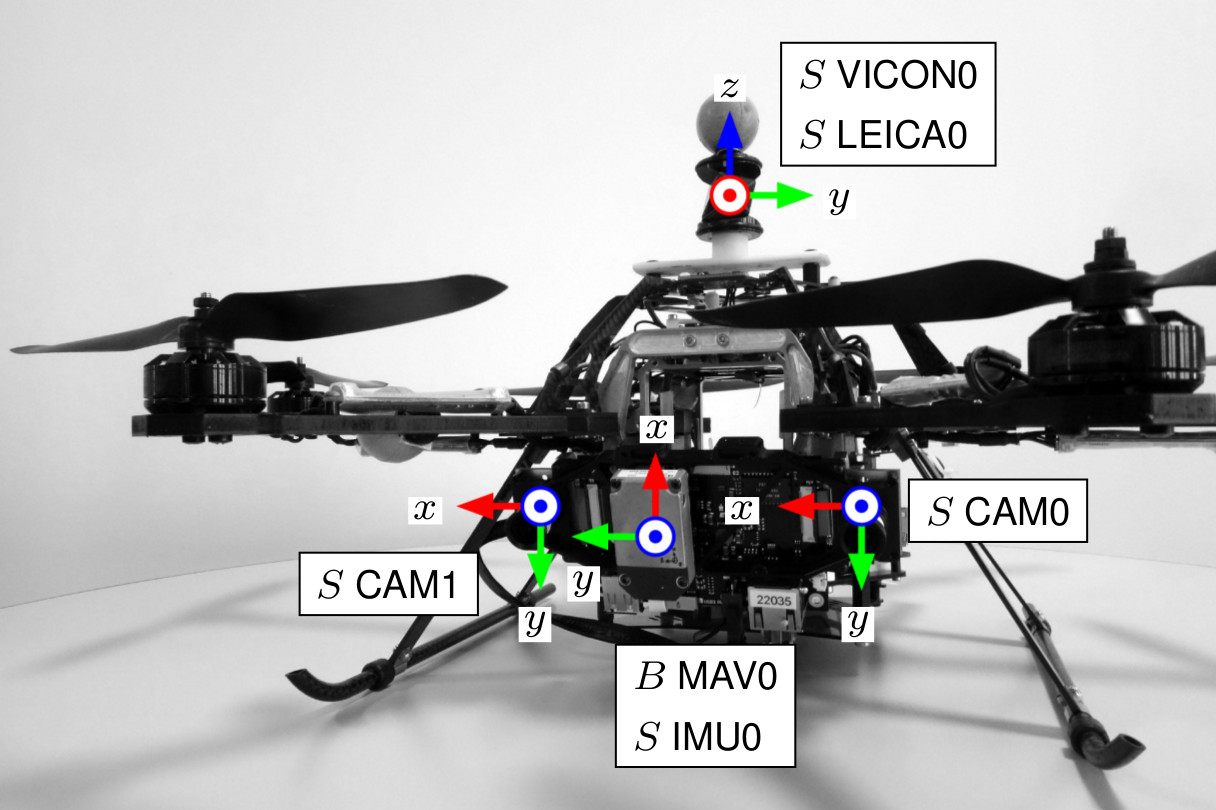
\includegraphics[width=\textwidth]{../img/euroc_platform.jpg}
    \caption[A micro aerial vehicle]{An Asctec Firefly hex-rotor micro aerial vehicle used for collecting the EuRoC micro aerial vehicle datasets. The picture shows reference frames of the sensors -- the stereo cameras and \gls{IMU}.}
    \label{fig:euroc_platform}
\end{figure}

\subsection{Dataset description}

The cameras produce a WVGA monochrome (greyscale) images at 20 frames per second. Cameras have a global shutter. The automatic exposure control is independent for both cameras. According to the published errata~\citep{Burri2016}, this ``resulted in different shutter times and in turn in different image brightnesses, rendering stereo matching and feature tracking more challenging''.

The dataset contains 11 mapping sessions in 3 different environments (``Machine Hall'', ``Vicon Room 1'', ``Vicon Room 2''). Each mapping session is available in a single \gls{ROS} bag file. First 5 sessions were captured in ETH machine hall (Figure~\ref{fig:eth-machine-hall}), a fairly large industrial environment featuring piping, reservoirs and many different types of surfaces. The second and the third batch of datasets were captured in a smaller furnished rectangular room. For the second and the third batch, the furnishing was different.

\begin{figure}
    \centering
    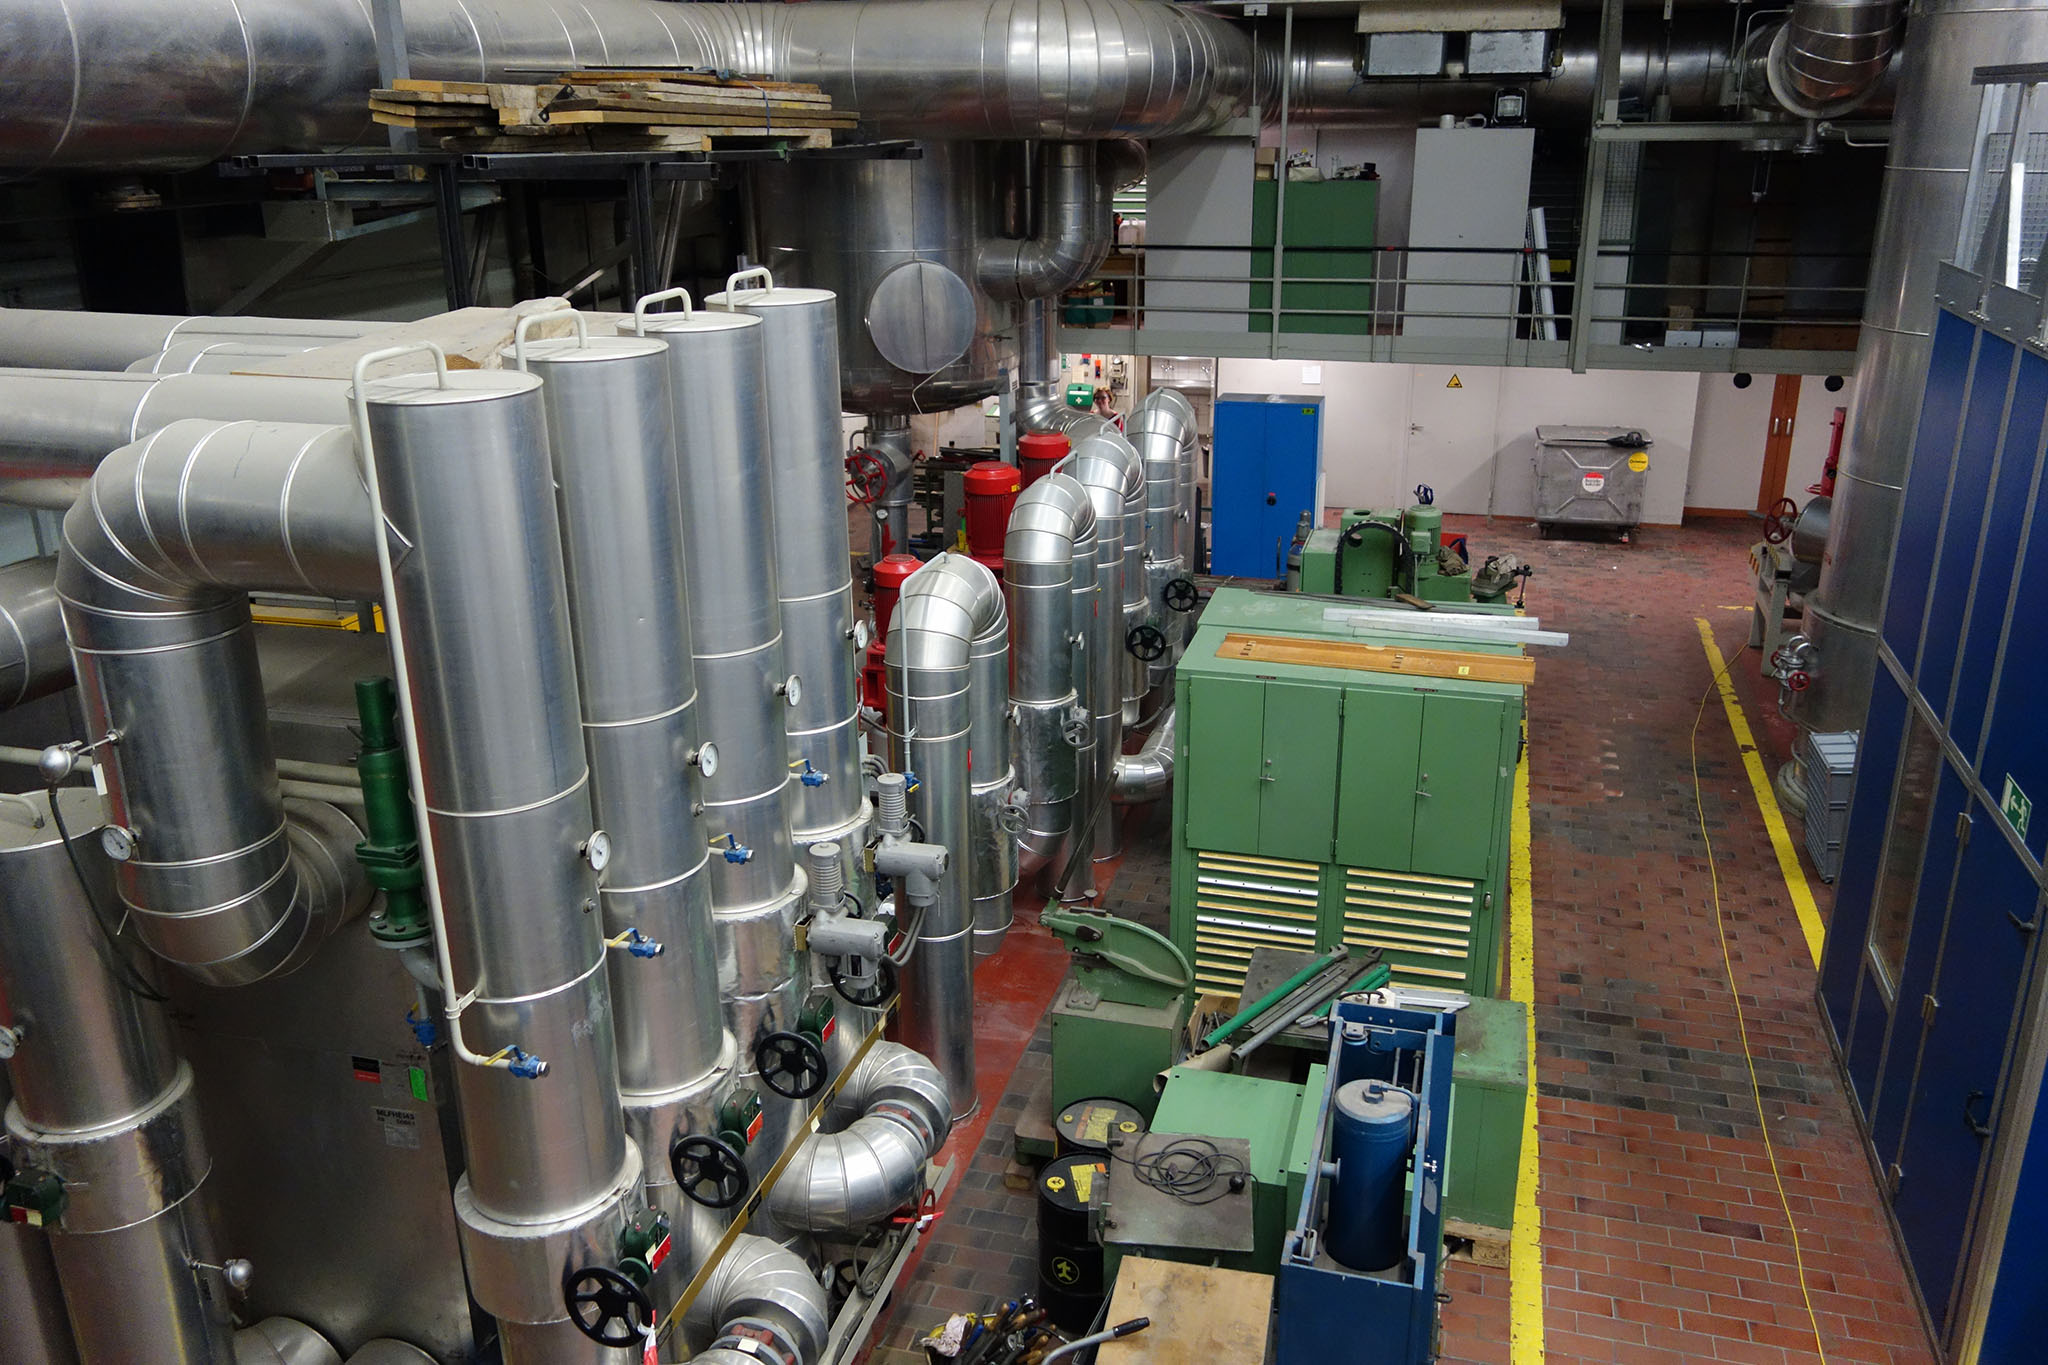
\includegraphics[width=\textwidth]{../img/eth_machine_room.jpg}
    \caption[ETH Machine hall]{ETH Machine hall industrial environment where $5$ mapping sessions of EuRoC dataset were captured. The image is courtesy of the authors~\citep{Burri2016}.}
    \label{fig:eth-machine-hall}
\end{figure}

\subsection{Maps generation}
\label{sec:euroc-generating-maps}

The dataset is intended for evaluating \gls{SLAM} algorithms, for our purposes, it was necessary to process the data with a \gls{SLAM} algorithm to create a point cloud maps.

First, I have used the provided calibration sequence and I have created a calibration data for \gls{ROS} using the \texttt{camera\_calibration} tool available with \gls{ROS}.

Second, for each environment, I created a pair of maps using the ``01'' and ``02'' mapping sessions from the datasets, which were used further for the evaluation of the map-merging (Figures~\ref{fig:euroc_mh_02}, \ref{fig:v1-greyscale}, \ref{fig:euroc_v2_02}).

Based on evaluations of \gls{SLAM} methods in \gls{ROS} done by~\citet{silva2017experimental} and \citet{ibragimov2017comparison}, I used RTAB-Map \gls{SLAM}, developed by~\citet{labbe2014online}, to create the maps. RTAB-Map can work with both stereo cameras and \gls{RGB-D} sensors and produces dense maps of good quality, as noted by both~\citet{silva2017experimental,ibragimov2017comparison}. ``RTAB-Map computed coherent SLAM solutions on all evaluated datasets and thus can be considered an efficient solution for 3D mapping scenarios'', summarise the results of RTAB-Map \citet{silva2017experimental}.

The odometry for mapping was provided from stereo camera data, using a visual odometry approach, the available \gls{IMU} data were not used. For the ``01'' sessions I have used a native visual odometry approach of RTAB-Map. For the ``02'' sessions I have used visual odometry approach of {ORB-SLAM2}, introduced by~\citet{mur2017orb}, because the data exhibit more dynamic motions, which lead to a frequent loss on visual odometry using the first approach. {ORB-SLAM2} visual odometry exhibited better robustness for this data. In both cases, a loop-closure approach of~\citet{labbe2014online} has been used.

The maps have been voxelized to the resolution of $0.05$ meters per voxel, which yields suitable map sizes for map exchange in a multi-robot system.

Using a different \gls{SLAM} pipeline for each of the maps contributed to introducing different mapping errors and artefacts, which makes map-merging of such maps more difficult.

\begin{figure}
    \centering
    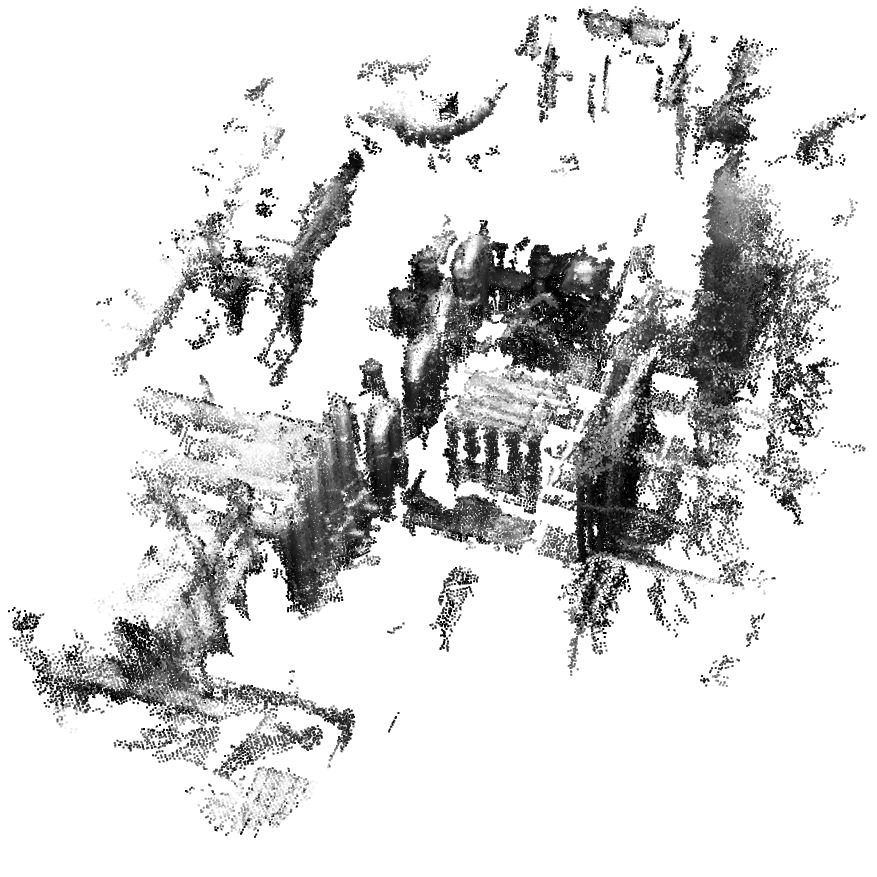
\includegraphics[width=\textwidth]{../img/euroc_mh_02.png}
    \caption[Machine hall point cloud map]{ETH Machine hall point cloud map. The map was produced from ``Machine Hall 02'' dataset using an {ORB-SLAM2} visual odometry~\citep{mur2017orb} and RTAB-Map loop-closure approach~\citep{labbe2014online}.}
    \label{fig:euroc_mh_02}
\end{figure}

\begin{figure}
    \centering
    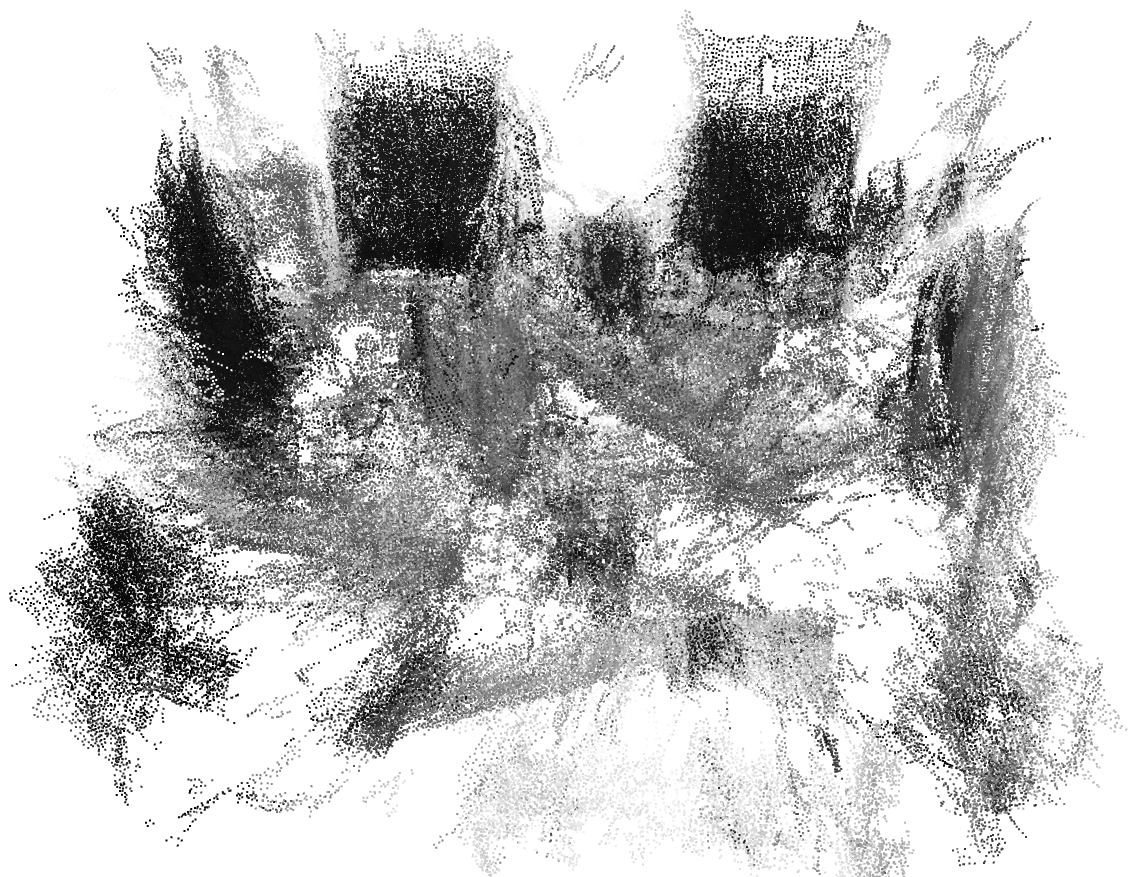
\includegraphics[width=\textwidth]{../img/euroc_v2_02.png}
    \caption[Point cloud map of a small room]{A point cloud map of a small room. The map was produced from ``Vicon Room 2 02'' dataset using an {ORB-SLAM2} visual odometry~\citep{mur2017orb} and RTAB-Map loop-closure approach~\citep{labbe2014online}.}
    \label{fig:euroc_v2_02}
\end{figure}

\section{AAU dataset}
\label{sec:aau-dataset}

The dataset recorded at \acrfull{AAU} on-board a micro aerial vehicle in an outdoor forest environment. The vehicle was equipped with a stereo camera rig and \gls{IMU}. The cameras produce greyscale images.

This dataset contains two mapping sessions. The environment consists or medium-sized trees, the ground is covered with leaves. The lighting conditions are challenging as there are areas of direct sunlight as well as areas in the shade. The lighting conditions are similar in both sessions, as the sessions were captured in the similar time of day. This setup causes difficult conditions for the stereo matching and the pose estimation, introducing mapping errors into the maps, which in turn make the map-merging a challenging task.

Maps (Figures~\ref{fig:aau_top}, \ref{fig:aau_lateral}) were generated in the similar manner as described in Section~\ref{sec:euroc-generating-maps}. Mapping has been done with RTAB-Map \gls{SLAM}~\citep{labbe2014online} using its native visual odometry approach.

% todo atribution

\begin{figure}
    \centering
    \begin{subfigure}[b]{0.82\textwidth}
        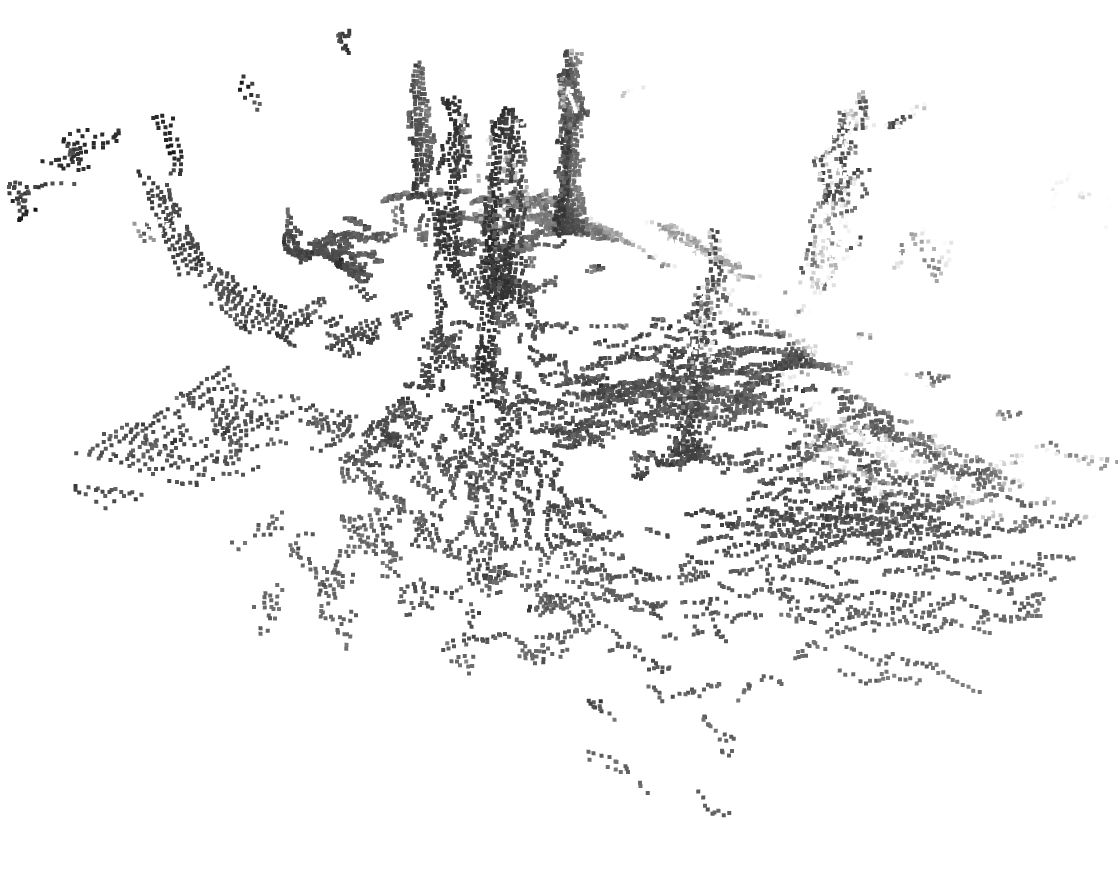
\includegraphics[width=\textwidth]{../img/aau_fc_dnav5_top.png}
        \caption{``\gls{AAU} forest 1'' map}
    \end{subfigure}
    % ~
    \begin{subfigure}[b]{0.82\textwidth}
        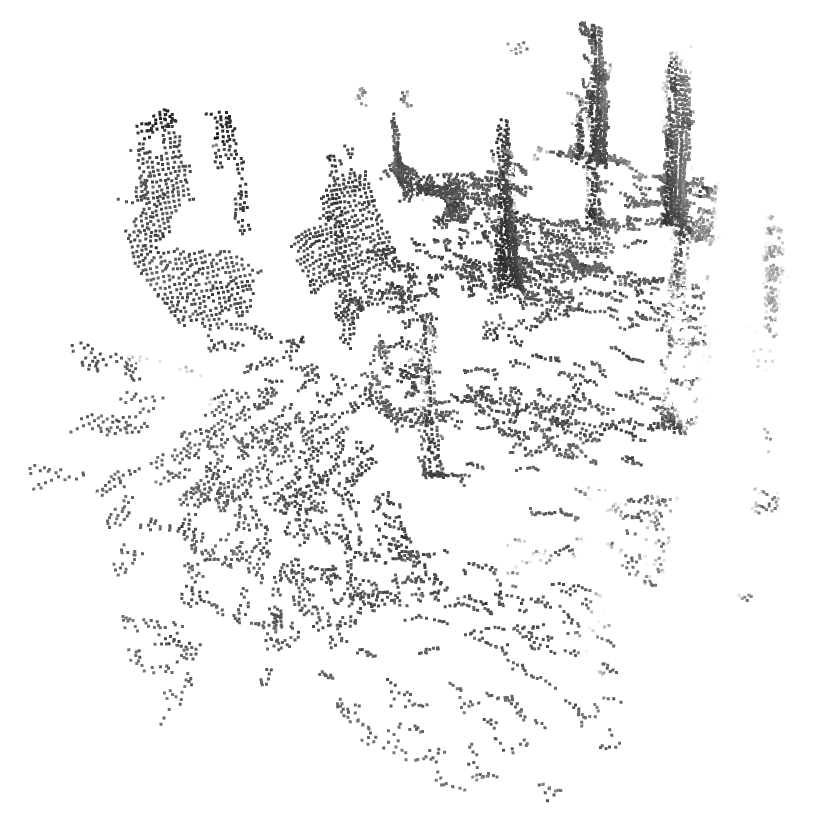
\includegraphics[width=\textwidth]{../img/aau_fc_dnav6_top.png}
        \caption{``\gls{AAU} forest 2'' map}
    \end{subfigure}
    \caption[Forest point cloud maps -- top view]{Top view of the two point cloud maps from \gls{AAU} outdoor forest dataset. Notice the stripe of direct sunlight on the ground causing difficult conditions for stereo matching.}
    \label{fig:aau_top}
\end{figure}

\begin{figure}
    \centering
    \begin{subfigure}[b]{\textwidth}
        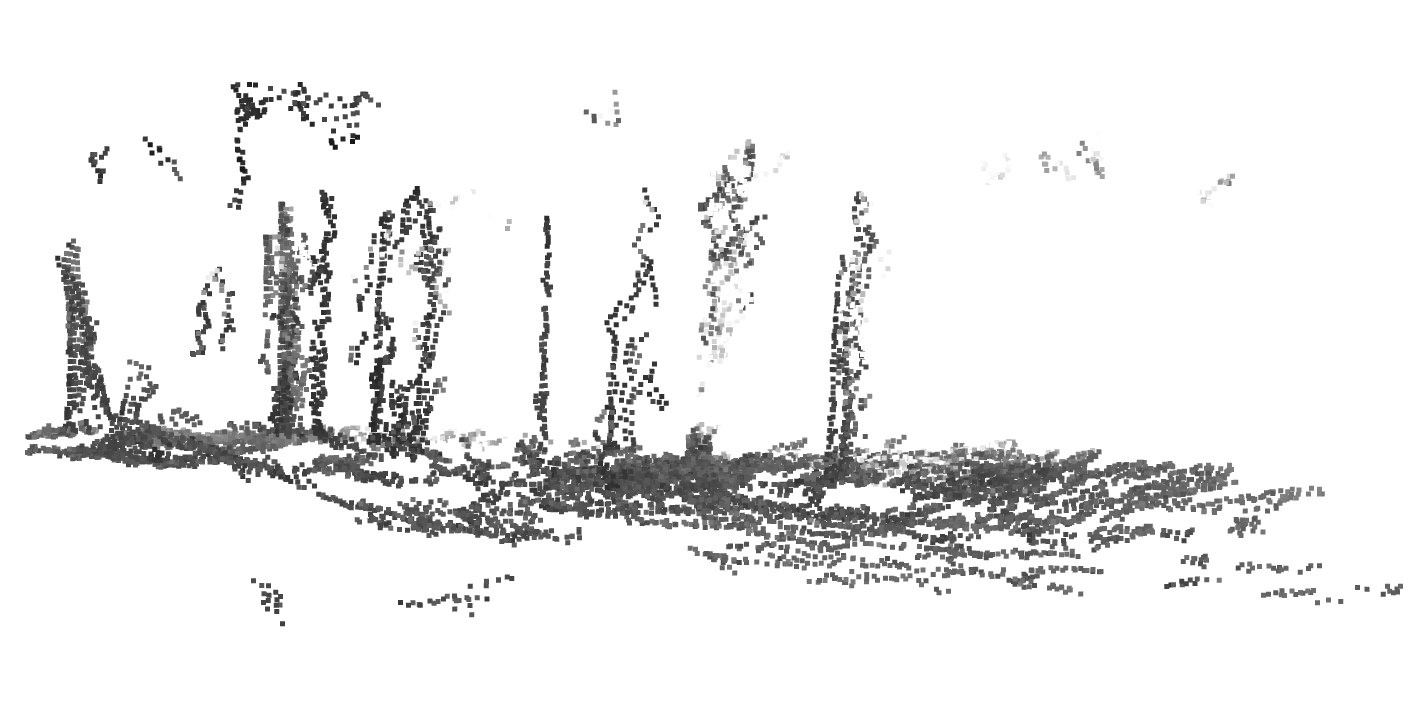
\includegraphics[width=\textwidth]{../img/aau_fc_dnav5_lateral.png}
        \caption{``\gls{AAU} forest 1'' map}
    \end{subfigure}
    % ~
    \begin{subfigure}[b]{\textwidth}
        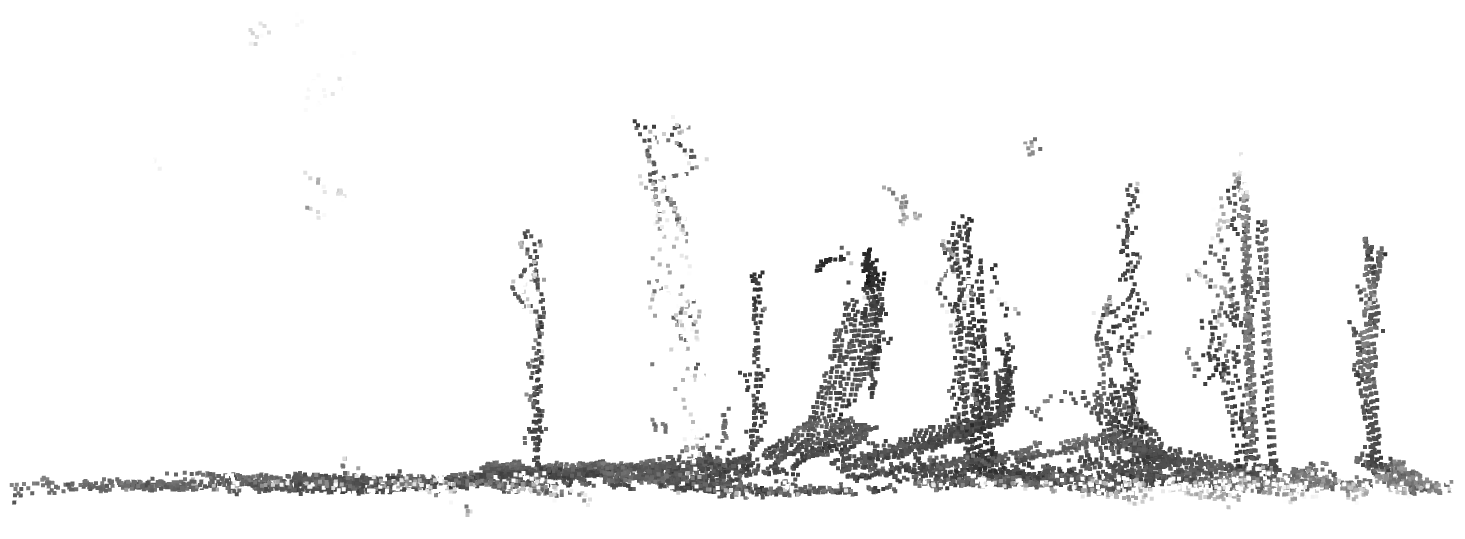
\includegraphics[width=\textwidth]{../img/aau_fc_dnav6_lateral.png}
        \caption{``\gls{AAU} forest 2'' map}
    \end{subfigure}
    \caption[Forest point cloud maps -- lateral view]{Lateral view of the two point cloud maps from \gls{AAU} outdoor forest dataset. In both maps there is a non-flat terrain and number of outliers caused by branches and difficult mapping conditions.}
    \label{fig:aau_lateral}
\end{figure}

\section{MFF dataset}
\label{sec:mff-dataset}

This dataset consists of my own experiments conducted at the campus of Faculty of Mathematics and Physics, Charles University. I have conducted two series of experiments.

The first series were using a handheld Orbbec Astra \gls{RGB-D} camera. I intended to create multi-floor maps of the campus building and evaluate this scenario with the map-merging algorithm. It has soon became apparent that without odometry source such mapping is challenging even for state of the art visual odometry approaches (Figure~\ref{fig:mff_second_third_floor}).

\begin{figure}
    \centering
    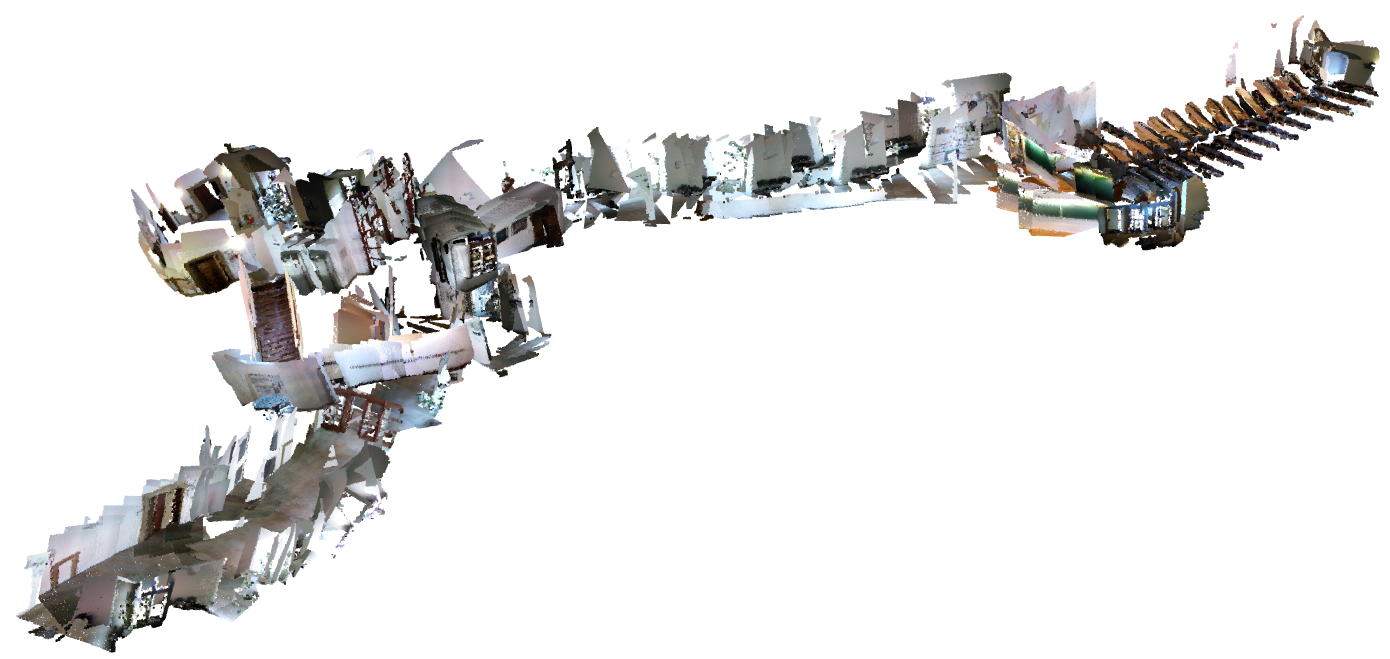
\includegraphics[width=\textwidth]{../img/mff_second_third_floor.png}
    \caption[A broken point cloud map of multiple campus floors]{The point cloud map of the second and third floor of the faculty building recorded during handheld mapping. The visual odometry was reset immediately after the tracking was lost. Due to frequent visual odometry failures the mapping attempt was not successful, although there are some partially consistent areas within the map.}
    \label{fig:mff_second_third_floor}
\end{figure}

Typically, during the mapping in narrow spaces, with difficult lighting conditions or during fast movements, the visual odometry tracking is lost and needs to be reset. Without the \gls{IMU} or any other external odometry source to bridge the loss of the visual odometry, it is hard to maintain a plausible odometry estimate. Two situations has been observed to be especially challenging for visual odometry approaches: rough movements (especially rotations) typical for handheld mapping, as humans tend to do less disciplined movements than robots, and transitions between spaces though narrow passages (e.g. doors), especially between spaces with different lighting conditions. Orbbec Astra camera does not contain an \gls{IMU} and, therefore, is less suitable for the handheld mapping, which typically exhibits rough movements.

Bridging the visual odometry gaps with \gls{SLAM} loop-closures is not always possible, especially for the second aforementioned type of errors. If the odometry is always lost when moving in and out of the specific room, such room became an isolated part of the \gls{SLAM} graph without any connections to the rest of the graph. Loop-closures between these two spaces connected by the narrow passage are very hard to achieve.

Because of the presented issues, I have conducted the second series of experiments with TurtleBot2 robot. It is a ground-based robot research platform designed to operate on flat surfaces.

The robot was equipped with Asus Xtion PRO \gls{RGB-D} camera, which was used for mapping, a gyroscope and wheel encoders providing \gls{2D} odometry.

The datasets used for evaluation were recorded in two different spaces ``Rotunda'', a half-circle computer laboratory with adjacent rooms (Figure~\ref{fig:mff_rotunda}), and ``Refectory'', containing a baroque refectory and lecture rooms at the first floor of the faculty building (Figure~\ref{fig:mff_refectory}). In each of the environments two maps were recorded.

\begin{figure}
    \centering
    \begin{subfigure}[b]{\textwidth}
        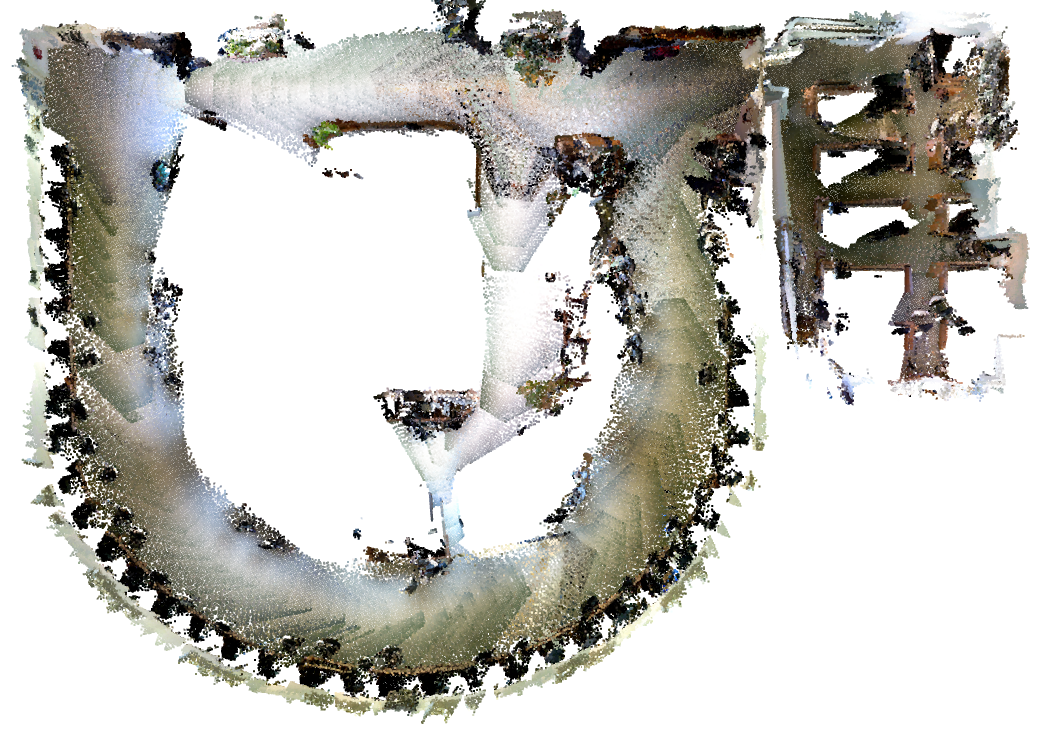
\includegraphics[width=\textwidth]{../img/mff_rotunda_1.png}
        \caption{``MFF Rotunda 1'' map}
    \end{subfigure}
    % ~
    \begin{subfigure}[b]{\textwidth}
        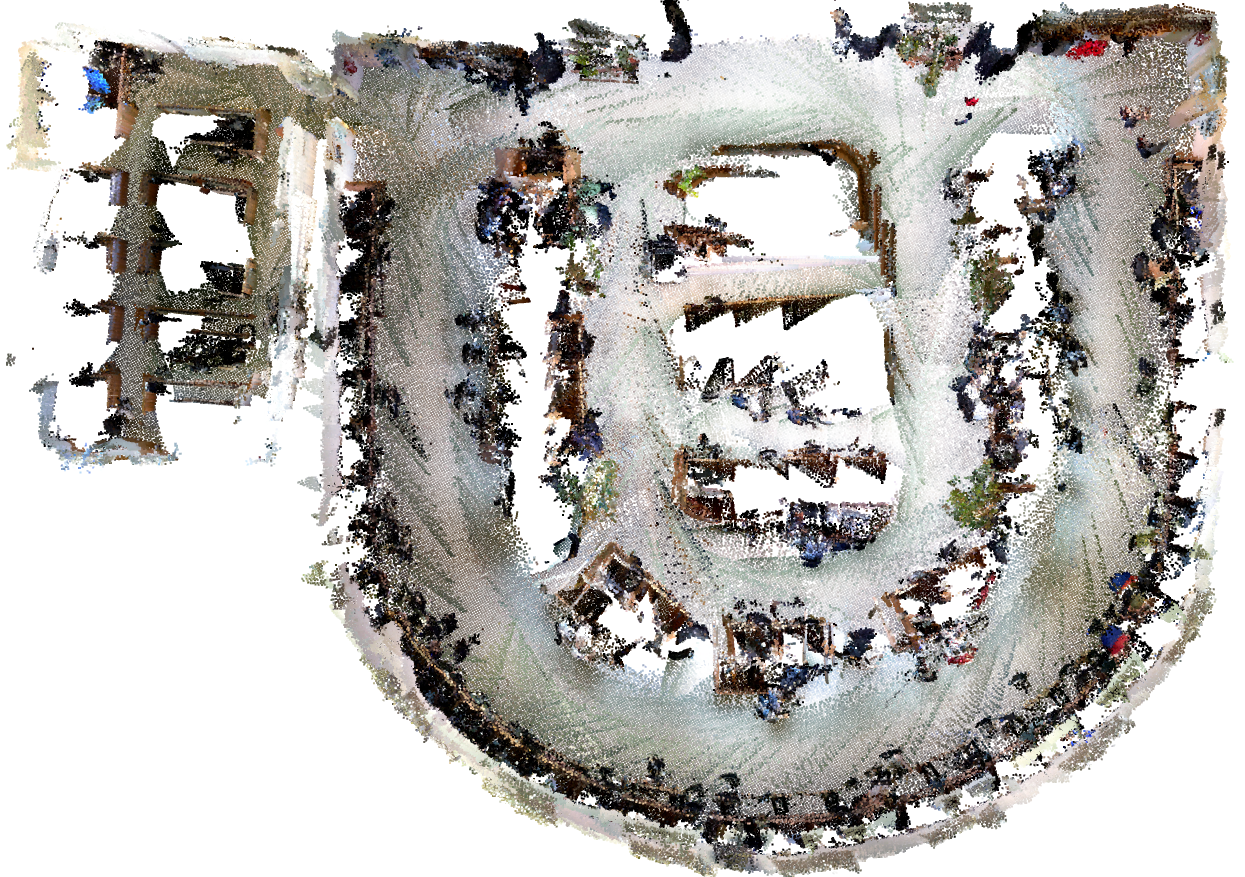
\includegraphics[width=\textwidth]{../img/mff_rotunda_2.png}
        \caption{``MFF Rotunda 2'' map}
    \end{subfigure}
    \caption[MFF Rotunda maps]{Maps of ``Rotunda'' computer laboratory with adjacent rooms recorded at the faculty building. The maps share a common mid-size area of a symmetrical half-circular laboratory. Both maps contain several mapping errors.}
    \label{fig:mff_rotunda}
\end{figure}

\begin{figure}
    \centering
    \begin{subfigure}[b]{0.65\textwidth}
        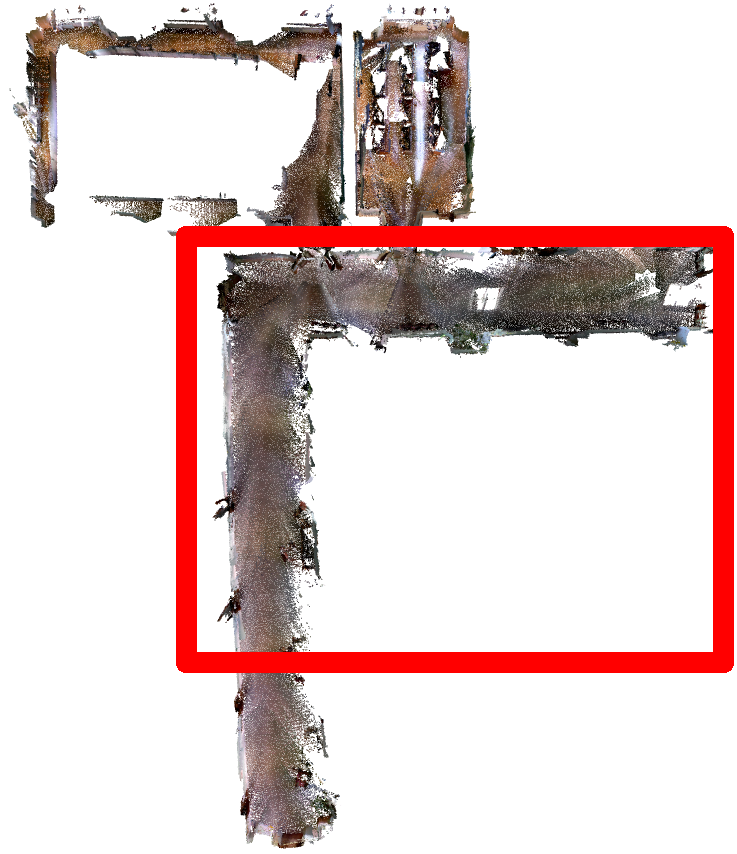
\includegraphics[width=\textwidth]{../img/mff_refectory_1_highlight.png}
        \caption{``MFF Refectory 1'' map}
    \end{subfigure}
    % ~
    \begin{subfigure}[b]{\textwidth}
        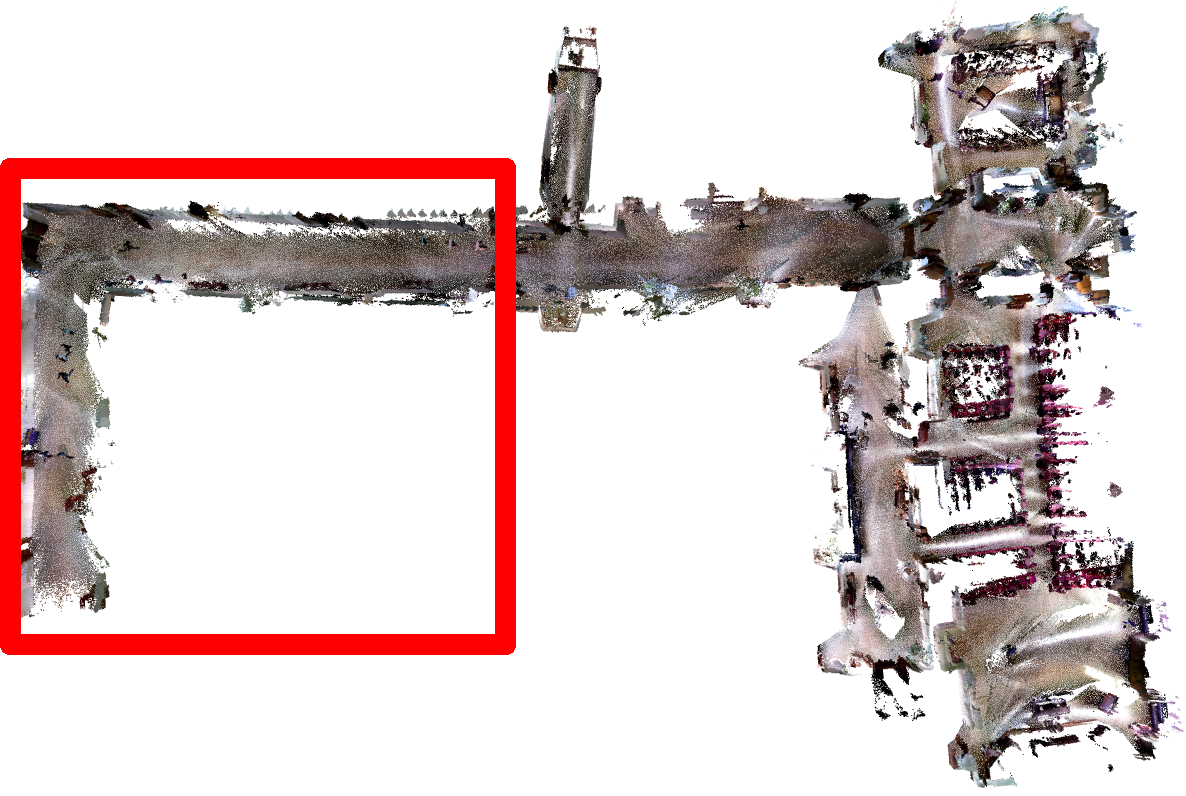
\includegraphics[width=\textwidth]{../img/mff_refectory_2_highlight.png}
        \caption{``MFF Refectory 2'' map}
    \end{subfigure}
    \caption[MFF Refectory maps]{Point cloud maps recorded at the first floor of the faculty building. The common area is highlighted. The larger map contains a baroque refectory with adjacent areas while the smaller map contains two lecture rooms. Notice the mapping errors in the corridor area, especially in the larger map.}
    \label{fig:mff_refectory}
\end{figure}


The maps were generated by RTAB-Map \gls{SLAM} as in the previous datasets. I used \gls{EKF} to fuse odometry data from the gyroscope, wheel encoders and the visual odometry provided by the native RTAB-Map approach. I used an \gls{EKF} implementation for \gls{ROS} by~\citet{moore2016ekf}. The filtering was using a \gls{2D} assumption as the robot operates in the plane. Together, those data provided a reliable odometry source for the \gls{SLAM} algorithm. The resulting maps were voxelized to the resolution of 0.05 meters per voxel. The maps are examined in Section~\ref{sec:mff-evaluation}.

\section{Accuracy}

For all the aerial datasets, the map-merging is able to correctly merge the maps. The Euclidean error scores, according to Section~\ref{sec:transform-evaluation}, are small across the datasets (Figure~\ref{fig:plot:euc_dist}). There are larger errors for the ``AAU forest'' and ``Machine Hall'' datasets caused by the outliers and mapping errors in those datasets, as those datasets have been recorded in tough conditions. Considering the artefacts in the datasets the alignment almost perfect and would allow precise coordination of the robots.

\begin{figure}
  \centering
  % GNUPLOT: LaTeX picture with Postscript
\begingroup
  \makeatletter
  \providecommand\color[2][]{%
    \GenericError{(gnuplot) \space\space\space\@spaces}{%
      Package color not loaded in conjunction with
      terminal option `colourtext'%
    }{See the gnuplot documentation for explanation.%
    }{Either use 'blacktext' in gnuplot or load the package
      color.sty in LaTeX.}%
    \renewcommand\color[2][]{}%
  }%
  \providecommand\includegraphics[2][]{%
    \GenericError{(gnuplot) \space\space\space\@spaces}{%
      Package graphicx or graphics not loaded%
    }{See the gnuplot documentation for explanation.%
    }{The gnuplot epslatex terminal needs graphicx.sty or graphics.sty.}%
    \renewcommand\includegraphics[2][]{}%
  }%
  \providecommand\rotatebox[2]{#2}%
  \@ifundefined{ifGPcolor}{%
    \newif\ifGPcolor
    \GPcolortrue
  }{}%
  \@ifundefined{ifGPblacktext}{%
    \newif\ifGPblacktext
    \GPblacktextfalse
  }{}%
  % define a \g@addto@macro without @ in the name:
  \let\gplgaddtomacro\g@addto@macro
  % define empty templates for all commands taking text:
  \gdef\gplbacktext{}%
  \gdef\gplfronttext{}%
  \makeatother
  \ifGPblacktext
    % no textcolor at all
    \def\colorrgb#1{}%
    \def\colorgray#1{}%
  \else
    % gray or color?
    \ifGPcolor
      \def\colorrgb#1{\color[rgb]{#1}}%
      \def\colorgray#1{\color[gray]{#1}}%
      \expandafter\def\csname LTw\endcsname{\color{white}}%
      \expandafter\def\csname LTb\endcsname{\color{black}}%
      \expandafter\def\csname LTa\endcsname{\color{black}}%
      \expandafter\def\csname LT0\endcsname{\color[rgb]{1,0,0}}%
      \expandafter\def\csname LT1\endcsname{\color[rgb]{0,1,0}}%
      \expandafter\def\csname LT2\endcsname{\color[rgb]{0,0,1}}%
      \expandafter\def\csname LT3\endcsname{\color[rgb]{1,0,1}}%
      \expandafter\def\csname LT4\endcsname{\color[rgb]{0,1,1}}%
      \expandafter\def\csname LT5\endcsname{\color[rgb]{1,1,0}}%
      \expandafter\def\csname LT6\endcsname{\color[rgb]{0,0,0}}%
      \expandafter\def\csname LT7\endcsname{\color[rgb]{1,0.3,0}}%
      \expandafter\def\csname LT8\endcsname{\color[rgb]{0.5,0.5,0.5}}%
    \else
      % gray
      \def\colorrgb#1{\color{black}}%
      \def\colorgray#1{\color[gray]{#1}}%
      \expandafter\def\csname LTw\endcsname{\color{white}}%
      \expandafter\def\csname LTb\endcsname{\color{black}}%
      \expandafter\def\csname LTa\endcsname{\color{black}}%
      \expandafter\def\csname LT0\endcsname{\color{black}}%
      \expandafter\def\csname LT1\endcsname{\color{black}}%
      \expandafter\def\csname LT2\endcsname{\color{black}}%
      \expandafter\def\csname LT3\endcsname{\color{black}}%
      \expandafter\def\csname LT4\endcsname{\color{black}}%
      \expandafter\def\csname LT5\endcsname{\color{black}}%
      \expandafter\def\csname LT6\endcsname{\color{black}}%
      \expandafter\def\csname LT7\endcsname{\color{black}}%
      \expandafter\def\csname LT8\endcsname{\color{black}}%
    \fi
  \fi
    \setlength{\unitlength}{0.0500bp}%
    \ifx\gptboxheight\undefined%
      \newlength{\gptboxheight}%
      \newlength{\gptboxwidth}%
      \newsavebox{\gptboxtext}%
    \fi%
    \setlength{\fboxrule}{0.5pt}%
    \setlength{\fboxsep}{1pt}%
\begin{picture}(8220.00,8220.00)%
    \gplgaddtomacro\gplbacktext{%
      \csname LTb\endcsname%%
      \put(747,1051){\makebox(0,0)[r]{\strut{}$0$}}%
      \csname LTb\endcsname%%
      \put(747,2142){\makebox(0,0)[r]{\strut{}$0.05$}}%
      \csname LTb\endcsname%%
      \put(747,3234){\makebox(0,0)[r]{\strut{}$0.1$}}%
      \csname LTb\endcsname%%
      \put(747,4325){\makebox(0,0)[r]{\strut{}$0.15$}}%
      \csname LTb\endcsname%%
      \put(747,5416){\makebox(0,0)[r]{\strut{}$0.2$}}%
      \csname LTb\endcsname%%
      \put(747,6508){\makebox(0,0)[r]{\strut{}$0.25$}}%
      \csname LTb\endcsname%%
      \put(747,7599){\makebox(0,0)[r]{\strut{}$0.3$}}%
      \csname LTb\endcsname%%
      \put(2262,949){\rotatebox{-45}{\makebox(0,0)[l]{\strut{}AAU forest}}}%
      \csname LTb\endcsname%%
      \put(3675,949){\rotatebox{-45}{\makebox(0,0)[l]{\strut{}Machine Hall}}}%
      \csname LTb\endcsname%%
      \put(5087,949){\rotatebox{-45}{\makebox(0,0)[l]{\strut{}Vicon Room 1}}}%
      \csname LTb\endcsname%%
      \put(6500,949){\rotatebox{-45}{\makebox(0,0)[l]{\strut{}Vicon Room 2}}}%
    }%
    \gplgaddtomacro\gplfronttext{%
      \csname LTb\endcsname%%
      \put(153,4325){\rotatebox{-270}{\makebox(0,0){\strut{}Distance (m)}}}%
      \csname LTb\endcsname%%
      \put(4381,7940){\makebox(0,0){\strut{}Euclidean error distance}}%
      \csname LTb\endcsname%%
      \put(7125,7432){\makebox(0,0)[r]{\strut{}MATCHING score}}%
      \csname LTb\endcsname%%
      \put(7125,7246){\makebox(0,0)[r]{\strut{}SAC-IA score}}%
      \csname LTb\endcsname%%
      \put(7125,7060){\makebox(0,0)[r]{\strut{}ICP score}}%
    }%
    \gplbacktext
    \put(0,0){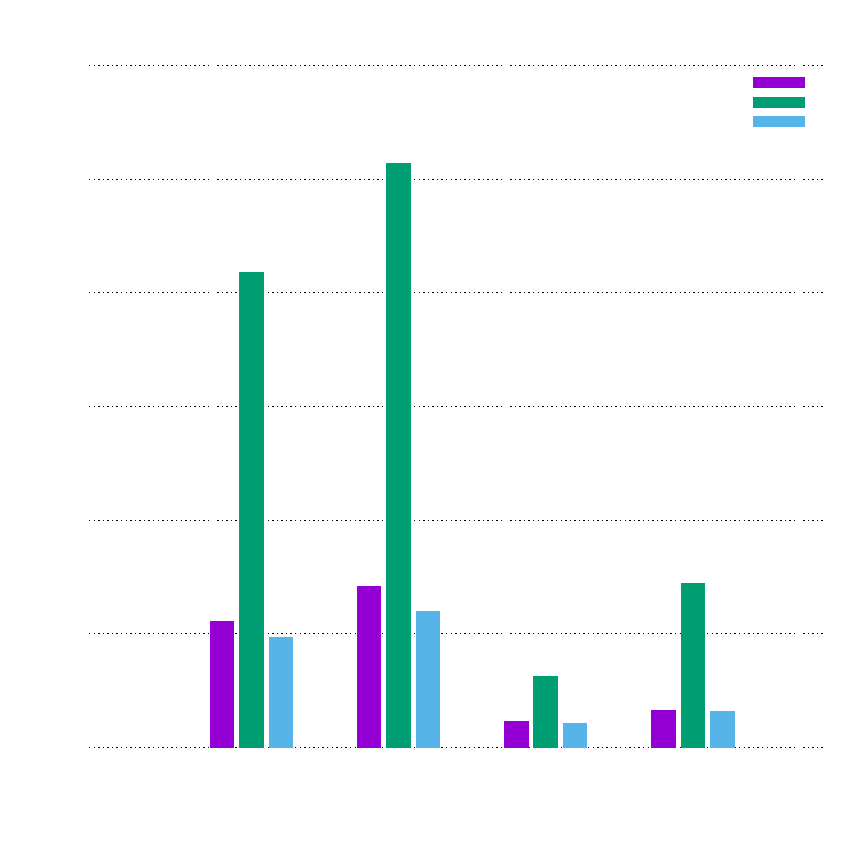
\includegraphics{euc_dist}}%
    \gplfronttext
  \end{picture}%
\endgroup

  \caption[Euclidean error scores for aerial datasets]{Euclidean error scores (sum of Euclidean distances for corresponding points) across the datasets. A threshold of $1.0$ has been used to cut-off fair laying point in non-overlapping areas, see Section~\ref{sec:transform-evaluation} for details. The map-merging run with default parameters including \gls{PFH} descriptors and \gls{SIFT} keypoints. The first two scores are for initial estimation using descriptors matching, using my reciprocal matching scheme and \gls{SAC-IA} algorithm respectively (Section~\ref{sec:matching}). The last score is the Euclidean error after final refining with \gls{ICP} (Section~\ref{sec:final-estimation}), the initial estimate from the reciprocal matching has been used for the \gls{ICP} refinement.}
  \label{fig:plot:euc_dist}
\end{figure}

Both ``Vicon Room'' datasets show very small Euclidean error, well beyond the size of one voxel ($0.05$ m). Considering the maps are down-sampled to the resolution of $0.1$ meters per voxel for the registration to allow merging of larger maps in real-world conditions, the presented algorithm can achieve a sub-voxel accuracy. The registration resolution of $0.1$ meters per voxel was used for all the evaluated maps.

The Euclidean error for the initial estimate is significantly lower for the presented reciprocal matching method (Section~\ref{sec:matching}). For the \gls{SAC-IA} algorithm, the error is higher because the randomness used in the algorithm introduces additional errors in case of well-performing \gls{PFH} descriptors. The initial estimate produced by the presented matching method is close to the final estimate refined with \gls{ICP}. The \gls{ICP} refinement is then very fast without negative impact on the overall time of the map-merging algorithm (Figure~\ref{fig:plot:perf}).

\section{Estimation robustness}

An important measure of estimation robustness is the number of inliers (Figure~\ref{fig:plot:inliers}) in the \gls{RANSAC} estimate (Section~\ref{sec:transform-evaluation}). Inliers are the points which are ultimately used for computing transformation estimate. Estimates based on a small number of inliers might be severely affected by the noise. On the other hand, estimates based on a large number of inliers, especially with the high inliers ratio to all points, are supposed to be reasonably confident in typical applications.

\begin{figure}
  \centering
  % GNUPLOT: LaTeX picture with Postscript
\begingroup
  \makeatletter
  \providecommand\color[2][]{%
    \GenericError{(gnuplot) \space\space\space\@spaces}{%
      Package color not loaded in conjunction with
      terminal option `colourtext'%
    }{See the gnuplot documentation for explanation.%
    }{Either use 'blacktext' in gnuplot or load the package
      color.sty in LaTeX.}%
    \renewcommand\color[2][]{}%
  }%
  \providecommand\includegraphics[2][]{%
    \GenericError{(gnuplot) \space\space\space\@spaces}{%
      Package graphicx or graphics not loaded%
    }{See the gnuplot documentation for explanation.%
    }{The gnuplot epslatex terminal needs graphicx.sty or graphics.sty.}%
    \renewcommand\includegraphics[2][]{}%
  }%
  \providecommand\rotatebox[2]{#2}%
  \@ifundefined{ifGPcolor}{%
    \newif\ifGPcolor
    \GPcolortrue
  }{}%
  \@ifundefined{ifGPblacktext}{%
    \newif\ifGPblacktext
    \GPblacktextfalse
  }{}%
  % define a \g@addto@macro without @ in the name:
  \let\gplgaddtomacro\g@addto@macro
  % define empty templates for all commands taking text:
  \gdef\gplbacktext{}%
  \gdef\gplfronttext{}%
  \makeatother
  \ifGPblacktext
    % no textcolor at all
    \def\colorrgb#1{}%
    \def\colorgray#1{}%
  \else
    % gray or color?
    \ifGPcolor
      \def\colorrgb#1{\color[rgb]{#1}}%
      \def\colorgray#1{\color[gray]{#1}}%
      \expandafter\def\csname LTw\endcsname{\color{white}}%
      \expandafter\def\csname LTb\endcsname{\color{black}}%
      \expandafter\def\csname LTa\endcsname{\color{black}}%
      \expandafter\def\csname LT0\endcsname{\color[rgb]{1,0,0}}%
      \expandafter\def\csname LT1\endcsname{\color[rgb]{0,1,0}}%
      \expandafter\def\csname LT2\endcsname{\color[rgb]{0,0,1}}%
      \expandafter\def\csname LT3\endcsname{\color[rgb]{1,0,1}}%
      \expandafter\def\csname LT4\endcsname{\color[rgb]{0,1,1}}%
      \expandafter\def\csname LT5\endcsname{\color[rgb]{1,1,0}}%
      \expandafter\def\csname LT6\endcsname{\color[rgb]{0,0,0}}%
      \expandafter\def\csname LT7\endcsname{\color[rgb]{1,0.3,0}}%
      \expandafter\def\csname LT8\endcsname{\color[rgb]{0.5,0.5,0.5}}%
    \else
      % gray
      \def\colorrgb#1{\color{black}}%
      \def\colorgray#1{\color[gray]{#1}}%
      \expandafter\def\csname LTw\endcsname{\color{white}}%
      \expandafter\def\csname LTb\endcsname{\color{black}}%
      \expandafter\def\csname LTa\endcsname{\color{black}}%
      \expandafter\def\csname LT0\endcsname{\color{black}}%
      \expandafter\def\csname LT1\endcsname{\color{black}}%
      \expandafter\def\csname LT2\endcsname{\color{black}}%
      \expandafter\def\csname LT3\endcsname{\color{black}}%
      \expandafter\def\csname LT4\endcsname{\color{black}}%
      \expandafter\def\csname LT5\endcsname{\color{black}}%
      \expandafter\def\csname LT6\endcsname{\color{black}}%
      \expandafter\def\csname LT7\endcsname{\color{black}}%
      \expandafter\def\csname LT8\endcsname{\color{black}}%
    \fi
  \fi
    \setlength{\unitlength}{0.0500bp}%
    \ifx\gptboxheight\undefined%
      \newlength{\gptboxheight}%
      \newlength{\gptboxwidth}%
      \newsavebox{\gptboxtext}%
    \fi%
    \setlength{\fboxrule}{0.5pt}%
    \setlength{\fboxsep}{1pt}%
\begin{picture}(8220.00,8220.00)%
    \gplgaddtomacro\gplbacktext{%
      \csname LTb\endcsname%%
      \put(459,1051){\makebox(0,0)[r]{\strut{}$0$}}%
      \csname LTb\endcsname%%
      \put(459,1646){\makebox(0,0)[r]{\strut{}$50$}}%
      \csname LTb\endcsname%%
      \put(459,2242){\makebox(0,0)[r]{\strut{}$100$}}%
      \csname LTb\endcsname%%
      \put(459,2837){\makebox(0,0)[r]{\strut{}$150$}}%
      \csname LTb\endcsname%%
      \put(459,3432){\makebox(0,0)[r]{\strut{}$200$}}%
      \csname LTb\endcsname%%
      \put(459,4027){\makebox(0,0)[r]{\strut{}$250$}}%
      \csname LTb\endcsname%%
      \put(459,4623){\makebox(0,0)[r]{\strut{}$300$}}%
      \csname LTb\endcsname%%
      \put(459,5218){\makebox(0,0)[r]{\strut{}$350$}}%
      \csname LTb\endcsname%%
      \put(459,5813){\makebox(0,0)[r]{\strut{}$400$}}%
      \csname LTb\endcsname%%
      \put(459,6408){\makebox(0,0)[r]{\strut{}$450$}}%
      \csname LTb\endcsname%%
      \put(459,7004){\makebox(0,0)[r]{\strut{}$500$}}%
      \csname LTb\endcsname%%
      \put(459,7599){\makebox(0,0)[r]{\strut{}$550$}}%
      \csname LTb\endcsname%%
      \put(2031,949){\rotatebox{-45}{\makebox(0,0)[l]{\strut{}AAU forest}}}%
      \csname LTb\endcsname%%
      \put(3502,949){\rotatebox{-45}{\makebox(0,0)[l]{\strut{}Machine Hall}}}%
      \csname LTb\endcsname%%
      \put(4972,949){\rotatebox{-45}{\makebox(0,0)[l]{\strut{}Vicon Room 1}}}%
      \csname LTb\endcsname%%
      \put(6443,949){\rotatebox{-45}{\makebox(0,0)[l]{\strut{}Vicon Room 2}}}%
    }%
    \gplgaddtomacro\gplfronttext{%
      \csname LTb\endcsname%%
      \put(4237,7940){\makebox(0,0){\strut{}Number of matches and inliers}}%
      \csname LTb\endcsname%%
      \put(7125,7432){\makebox(0,0)[r]{\strut{}cross-matches count}}%
      \csname LTb\endcsname%%
      \put(7125,7246){\makebox(0,0)[r]{\strut{}inliers count}}%
      \csname LTb\endcsname%%
      \put(2378,1392){\makebox(0,0){\strut{}13}}%
      \csname LTb\endcsname%%
      \put(3849,1511){\makebox(0,0){\strut{}23}}%
      \csname LTb\endcsname%%
      \put(5319,1666){\makebox(0,0){\strut{}36}}%
      \csname LTb\endcsname%%
      \put(6790,1356){\makebox(0,0){\strut{}10}}%
    }%
    \gplbacktext
    \put(0,0){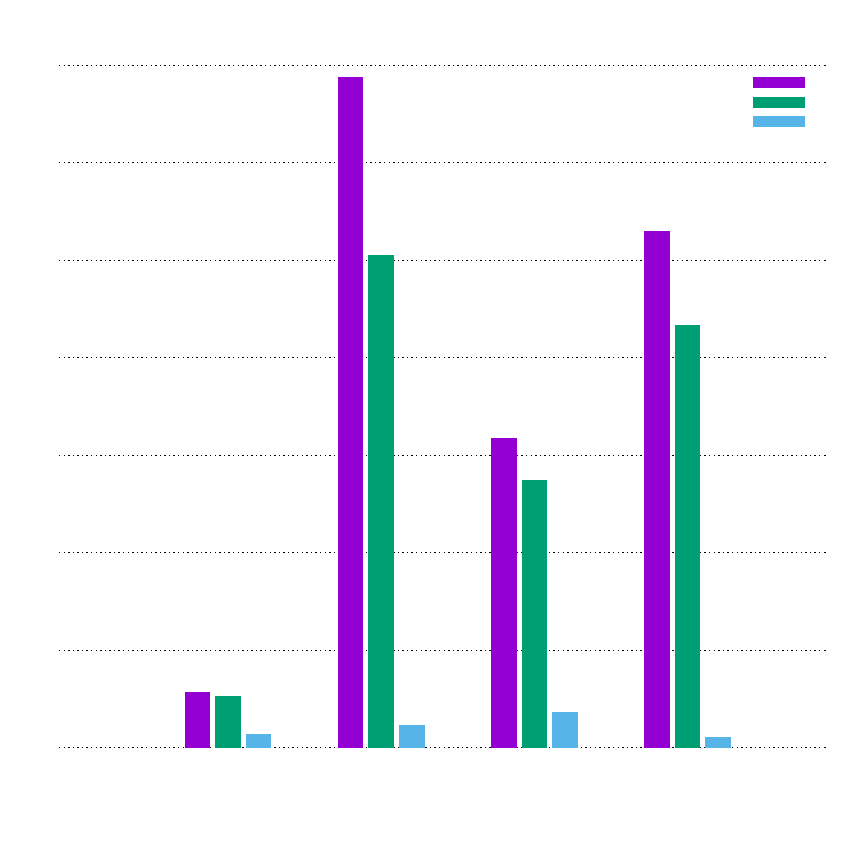
\includegraphics{inliers}}%
    \gplfronttext
  \end{picture}%
\endgroup

  \caption[Number of keypoints, matches and inliers for aerial datasets]{Number of keypoints, descriptor matches and number of inliers across the datasets with default parameters. Default parameters include \gls{PFH} descriptors and \gls{SIFT} keypoints. The reciprocal matching algorithm (Section~\ref{sec:matching}) has been used for matching. Keypoints are shown for the first map of each environment.}
  \label{fig:plot:inliers}
\end{figure}

The inlier ratio (the number of matches to the number of inliers) is quite low, even for \gls{PFH} descriptors (Figure~\ref{fig:plot:inliers}), the similar ratios have been observed for all the descriptors. This is partially caused by the matching scheme designed to accept also more distant matches to improve inlier ratio for less descriptive descriptors as discussed in Section~\ref{sec:matching}. The same behaviour causes the number of matches to be relatively high compared to the number of keypoints (Figure~\ref{fig:plot:inliers}).

The ``AAU forest'' and ``Vicon Room 2'' datasets have low numbers of inliers, which might impact robustness in such environments. The ``AAU forest'' is a relatively small, difficult environment for mapping containing noise and mapping errors. Only a few regions in maps are suitable for producing reliable matching points, which leads to the small number of inliers.

For the ``Vicon Room 2'' dataset colour-based descriptors exhibited generally better performance (Figure~\ref{fig:plot:desc_inliers}) allow robust estimation for this dataset. The ``Vicon Room 2'' maps also contain noise caused by the dynamic motion of the aerial vehicle.

Interestingly in both cases with a limited number of inliers, the map-merging algorithm has been able to produce an accurate merge (Figure~\ref{fig:plot:euc_dist}), even before \gls{ICP} refining. The inliers proved to be the correct matches.

\section{Descriptors}

As already noted in the previous section, the performance of the descriptors varies significantly in some cases (Figure~\ref{fig:plot:desc_inliers}). The \gls{PFHRGB} descriptors exhibited the highest number of inliers across the datasets (Figure~\ref{fig:plot:desc_inliers}). The \gls{SHOT} descriptors with colour also exhibited a decent amount of inliers, especially considering the fast processing speed (Section~\ref{sec:runtime-perf}).

\begin{figure}
  \centering
  % GNUPLOT: LaTeX picture with Postscript
\begingroup
  \makeatletter
  \providecommand\color[2][]{%
    \GenericError{(gnuplot) \space\space\space\@spaces}{%
      Package color not loaded in conjunction with
      terminal option `colourtext'%
    }{See the gnuplot documentation for explanation.%
    }{Either use 'blacktext' in gnuplot or load the package
      color.sty in LaTeX.}%
    \renewcommand\color[2][]{}%
  }%
  \providecommand\includegraphics[2][]{%
    \GenericError{(gnuplot) \space\space\space\@spaces}{%
      Package graphicx or graphics not loaded%
    }{See the gnuplot documentation for explanation.%
    }{The gnuplot epslatex terminal needs graphicx.sty or graphics.sty.}%
    \renewcommand\includegraphics[2][]{}%
  }%
  \providecommand\rotatebox[2]{#2}%
  \@ifundefined{ifGPcolor}{%
    \newif\ifGPcolor
    \GPcolortrue
  }{}%
  \@ifundefined{ifGPblacktext}{%
    \newif\ifGPblacktext
    \GPblacktextfalse
  }{}%
  % define a \g@addto@macro without @ in the name:
  \let\gplgaddtomacro\g@addto@macro
  % define empty templates for all commands taking text:
  \gdef\gplbacktext{}%
  \gdef\gplfronttext{}%
  \makeatother
  \ifGPblacktext
    % no textcolor at all
    \def\colorrgb#1{}%
    \def\colorgray#1{}%
  \else
    % gray or color?
    \ifGPcolor
      \def\colorrgb#1{\color[rgb]{#1}}%
      \def\colorgray#1{\color[gray]{#1}}%
      \expandafter\def\csname LTw\endcsname{\color{white}}%
      \expandafter\def\csname LTb\endcsname{\color{black}}%
      \expandafter\def\csname LTa\endcsname{\color{black}}%
      \expandafter\def\csname LT0\endcsname{\color[rgb]{1,0,0}}%
      \expandafter\def\csname LT1\endcsname{\color[rgb]{0,1,0}}%
      \expandafter\def\csname LT2\endcsname{\color[rgb]{0,0,1}}%
      \expandafter\def\csname LT3\endcsname{\color[rgb]{1,0,1}}%
      \expandafter\def\csname LT4\endcsname{\color[rgb]{0,1,1}}%
      \expandafter\def\csname LT5\endcsname{\color[rgb]{1,1,0}}%
      \expandafter\def\csname LT6\endcsname{\color[rgb]{0,0,0}}%
      \expandafter\def\csname LT7\endcsname{\color[rgb]{1,0.3,0}}%
      \expandafter\def\csname LT8\endcsname{\color[rgb]{0.5,0.5,0.5}}%
    \else
      % gray
      \def\colorrgb#1{\color{black}}%
      \def\colorgray#1{\color[gray]{#1}}%
      \expandafter\def\csname LTw\endcsname{\color{white}}%
      \expandafter\def\csname LTb\endcsname{\color{black}}%
      \expandafter\def\csname LTa\endcsname{\color{black}}%
      \expandafter\def\csname LT0\endcsname{\color{black}}%
      \expandafter\def\csname LT1\endcsname{\color{black}}%
      \expandafter\def\csname LT2\endcsname{\color{black}}%
      \expandafter\def\csname LT3\endcsname{\color{black}}%
      \expandafter\def\csname LT4\endcsname{\color{black}}%
      \expandafter\def\csname LT5\endcsname{\color{black}}%
      \expandafter\def\csname LT6\endcsname{\color{black}}%
      \expandafter\def\csname LT7\endcsname{\color{black}}%
      \expandafter\def\csname LT8\endcsname{\color{black}}%
    \fi
  \fi
    \setlength{\unitlength}{0.0500bp}%
    \ifx\gptboxheight\undefined%
      \newlength{\gptboxheight}%
      \newlength{\gptboxwidth}%
      \newsavebox{\gptboxtext}%
    \fi%
    \setlength{\fboxrule}{0.5pt}%
    \setlength{\fboxsep}{1pt}%
\begin{picture}(8220.00,8220.00)%
    \gplgaddtomacro\gplbacktext{%
      \csname LTb\endcsname%%
      \put(357,1051){\makebox(0,0)[r]{\strut{}$0$}}%
      \csname LTb\endcsname%%
      \put(357,1779){\makebox(0,0)[r]{\strut{}$5$}}%
      \csname LTb\endcsname%%
      \put(357,2506){\makebox(0,0)[r]{\strut{}$10$}}%
      \csname LTb\endcsname%%
      \put(357,3234){\makebox(0,0)[r]{\strut{}$15$}}%
      \csname LTb\endcsname%%
      \put(357,3961){\makebox(0,0)[r]{\strut{}$20$}}%
      \csname LTb\endcsname%%
      \put(357,4689){\makebox(0,0)[r]{\strut{}$25$}}%
      \csname LTb\endcsname%%
      \put(357,5416){\makebox(0,0)[r]{\strut{}$30$}}%
      \csname LTb\endcsname%%
      \put(357,6144){\makebox(0,0)[r]{\strut{}$35$}}%
      \csname LTb\endcsname%%
      \put(357,6871){\makebox(0,0)[r]{\strut{}$40$}}%
      \csname LTb\endcsname%%
      \put(357,7599){\makebox(0,0)[r]{\strut{}$45$}}%
      \csname LTb\endcsname%%
      \put(1950,949){\rotatebox{-45}{\makebox(0,0)[l]{\strut{}AAU forest}}}%
      \csname LTb\endcsname%%
      \put(3441,949){\rotatebox{-45}{\makebox(0,0)[l]{\strut{}Machine Hall}}}%
      \csname LTb\endcsname%%
      \put(4931,949){\rotatebox{-45}{\makebox(0,0)[l]{\strut{}Vicon Room 1}}}%
      \csname LTb\endcsname%%
      \put(6422,949){\rotatebox{-45}{\makebox(0,0)[l]{\strut{}Vicon Room 2}}}%
    }%
    \gplgaddtomacro\gplfronttext{%
      \csname LTb\endcsname%%
      \put(4186,7940){\makebox(0,0){\strut{}Number of inliers per descriptor}}%
      \csname LTb\endcsname%%
      \put(1173,7432){\makebox(0,0)[r]{\strut{}FPFH}}%
      \csname LTb\endcsname%%
      \put(1173,7246){\makebox(0,0)[r]{\strut{}PFH}}%
      \csname LTb\endcsname%%
      \put(1173,7060){\makebox(0,0)[r]{\strut{}PFHRGB}}%
      \csname LTb\endcsname%%
      \put(1173,6874){\makebox(0,0)[r]{\strut{}SC3D}}%
      \csname LTb\endcsname%%
      \put(1173,6688){\makebox(0,0)[r]{\strut{}SHOT}}%
    }%
    \gplbacktext
    \put(0,0){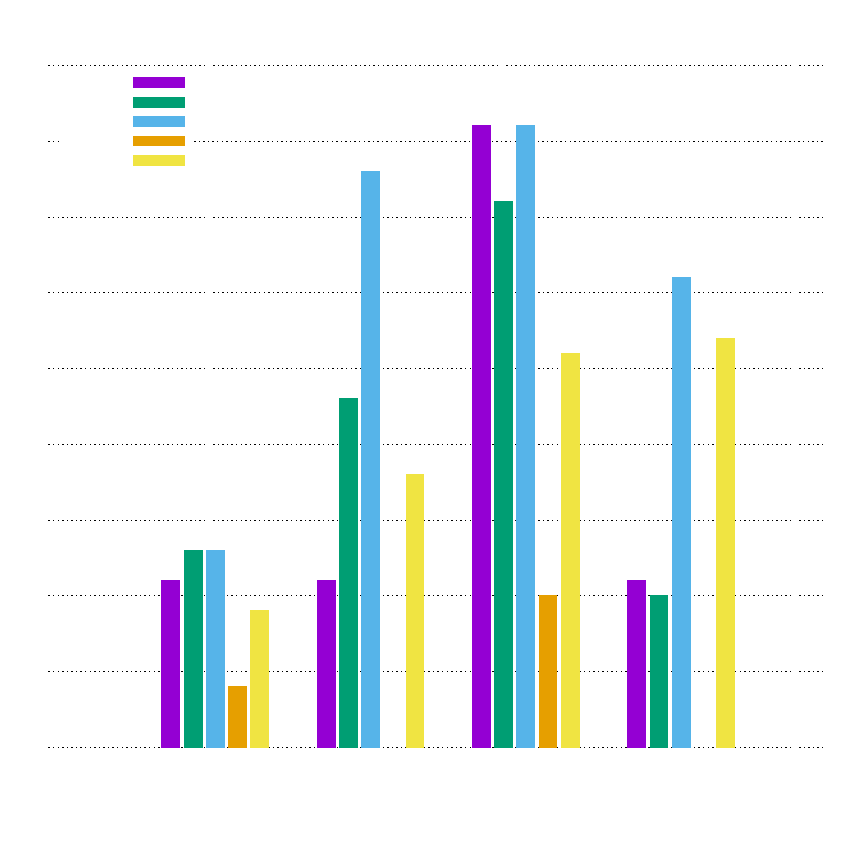
\includegraphics{desc_inliers}}%
    \gplfronttext
  \end{picture}%
\endgroup

  \caption[Number of inliers per descriptors]{Number of inliers across the datasets for different descriptor algorithms. Apart from descriptors algorithms, the default parameters has been used including \gls{SIFT} keypoints and the reciprocal matching algorithm (Section~\ref{sec:matching}). The \gls{PCL} implementation of \gls{SC3D} descriptors crashed on ``Machine Hall'' and ``Vicon Room 2'' datasets. This might indicate that the implementation in \gls{PCL} is probably not as mature as the remaining descriptors, but I have not investigated further.}
  \label{fig:plot:desc_inliers}
\end{figure}

The lowest number of inliers have been produced by \gls{SC3D} descriptors. Moreover, the \gls{PCL} implementation of \gls{SC3D} crashed in two instances. Together with \gls{RSD} descriptors, which has not been able to produce any inliers and are not shown in the plots, the \gls{SC3D} may not be suitable for map-merging in the evaluated setup.

Euclidean error distances (Figure~\ref{fig:plot:desc_dist}) mostly reflects the number of inliers for respective descriptors, with \gls{PFHRGB} descriptors generally providing the best initial transformation. With one exception, the \gls{ICP} refining was able to produce high-quality alignment for all descriptors with small error differences, neglecting the differences between initial alignments for different descriptors. For the \gls{FPFH} descriptors, the initial estimate in ``Machine Hall'' dataset has a significantly higher error and the \gls{ICP} refining stuck in the local extreme.

\begin{figure}
  \centering
  % GNUPLOT: LaTeX picture with Postscript
\begingroup
  \makeatletter
  \providecommand\color[2][]{%
    \GenericError{(gnuplot) \space\space\space\@spaces}{%
      Package color not loaded in conjunction with
      terminal option `colourtext'%
    }{See the gnuplot documentation for explanation.%
    }{Either use 'blacktext' in gnuplot or load the package
      color.sty in LaTeX.}%
    \renewcommand\color[2][]{}%
  }%
  \providecommand\includegraphics[2][]{%
    \GenericError{(gnuplot) \space\space\space\@spaces}{%
      Package graphicx or graphics not loaded%
    }{See the gnuplot documentation for explanation.%
    }{The gnuplot epslatex terminal needs graphicx.sty or graphics.sty.}%
    \renewcommand\includegraphics[2][]{}%
  }%
  \providecommand\rotatebox[2]{#2}%
  \@ifundefined{ifGPcolor}{%
    \newif\ifGPcolor
    \GPcolortrue
  }{}%
  \@ifundefined{ifGPblacktext}{%
    \newif\ifGPblacktext
    \GPblacktextfalse
  }{}%
  % define a \g@addto@macro without @ in the name:
  \let\gplgaddtomacro\g@addto@macro
  % define empty templates for all commands taking text:
  \gdef\gplbacktext{}%
  \gdef\gplfronttext{}%
  \makeatother
  \ifGPblacktext
    % no textcolor at all
    \def\colorrgb#1{}%
    \def\colorgray#1{}%
  \else
    % gray or color?
    \ifGPcolor
      \def\colorrgb#1{\color[rgb]{#1}}%
      \def\colorgray#1{\color[gray]{#1}}%
      \expandafter\def\csname LTw\endcsname{\color{white}}%
      \expandafter\def\csname LTb\endcsname{\color{black}}%
      \expandafter\def\csname LTa\endcsname{\color{black}}%
      \expandafter\def\csname LT0\endcsname{\color[rgb]{1,0,0}}%
      \expandafter\def\csname LT1\endcsname{\color[rgb]{0,1,0}}%
      \expandafter\def\csname LT2\endcsname{\color[rgb]{0,0,1}}%
      \expandafter\def\csname LT3\endcsname{\color[rgb]{1,0,1}}%
      \expandafter\def\csname LT4\endcsname{\color[rgb]{0,1,1}}%
      \expandafter\def\csname LT5\endcsname{\color[rgb]{1,1,0}}%
      \expandafter\def\csname LT6\endcsname{\color[rgb]{0,0,0}}%
      \expandafter\def\csname LT7\endcsname{\color[rgb]{1,0.3,0}}%
      \expandafter\def\csname LT8\endcsname{\color[rgb]{0.5,0.5,0.5}}%
    \else
      % gray
      \def\colorrgb#1{\color{black}}%
      \def\colorgray#1{\color[gray]{#1}}%
      \expandafter\def\csname LTw\endcsname{\color{white}}%
      \expandafter\def\csname LTb\endcsname{\color{black}}%
      \expandafter\def\csname LTa\endcsname{\color{black}}%
      \expandafter\def\csname LT0\endcsname{\color{black}}%
      \expandafter\def\csname LT1\endcsname{\color{black}}%
      \expandafter\def\csname LT2\endcsname{\color{black}}%
      \expandafter\def\csname LT3\endcsname{\color{black}}%
      \expandafter\def\csname LT4\endcsname{\color{black}}%
      \expandafter\def\csname LT5\endcsname{\color{black}}%
      \expandafter\def\csname LT6\endcsname{\color{black}}%
      \expandafter\def\csname LT7\endcsname{\color{black}}%
      \expandafter\def\csname LT8\endcsname{\color{black}}%
    \fi
  \fi
    \setlength{\unitlength}{0.0500bp}%
    \ifx\gptboxheight\undefined%
      \newlength{\gptboxheight}%
      \newlength{\gptboxwidth}%
      \newsavebox{\gptboxtext}%
    \fi%
    \setlength{\fboxrule}{0.5pt}%
    \setlength{\fboxsep}{1pt}%
\begin{picture}(8220.00,8220.00)%
    \gplgaddtomacro\gplbacktext{%
      \csname LTb\endcsname%%
      \put(747,1051){\makebox(0,0)[r]{\strut{}$0$}}%
      \csname LTb\endcsname%%
      \put(747,1986){\makebox(0,0)[r]{\strut{}$0.05$}}%
      \csname LTb\endcsname%%
      \put(747,2922){\makebox(0,0)[r]{\strut{}$0.1$}}%
      \csname LTb\endcsname%%
      \put(747,3857){\makebox(0,0)[r]{\strut{}$0.15$}}%
      \csname LTb\endcsname%%
      \put(747,4793){\makebox(0,0)[r]{\strut{}$0.2$}}%
      \csname LTb\endcsname%%
      \put(747,5728){\makebox(0,0)[r]{\strut{}$0.25$}}%
      \csname LTb\endcsname%%
      \put(747,6664){\makebox(0,0)[r]{\strut{}$0.3$}}%
      \csname LTb\endcsname%%
      \put(747,7599){\makebox(0,0)[r]{\strut{}$0.35$}}%
      \csname LTb\endcsname%%
      \put(2262,949){\rotatebox{-45}{\makebox(0,0)[l]{\strut{}AAU forest}}}%
      \csname LTb\endcsname%%
      \put(3675,949){\rotatebox{-45}{\makebox(0,0)[l]{\strut{}Machine Hall}}}%
      \csname LTb\endcsname%%
      \put(5087,949){\rotatebox{-45}{\makebox(0,0)[l]{\strut{}Vicon Room 1}}}%
      \csname LTb\endcsname%%
      \put(6500,949){\rotatebox{-45}{\makebox(0,0)[l]{\strut{}Vicon Room 2}}}%
    }%
    \gplgaddtomacro\gplfronttext{%
      \csname LTb\endcsname%%
      \put(153,4325){\rotatebox{-270}{\makebox(0,0){\strut{}Distance (m)}}}%
      \csname LTb\endcsname%%
      \put(4381,7940){\makebox(0,0){\strut{}Euclidean error distance for descriptors}}%
      \csname LTb\endcsname%%
      \put(7125,7432){\makebox(0,0)[r]{\strut{}FPFH}}%
      \csname LTb\endcsname%%
      \put(7125,7246){\makebox(0,0)[r]{\strut{}PFH}}%
      \csname LTb\endcsname%%
      \put(7125,7060){\makebox(0,0)[r]{\strut{}PFHRGB}}%
      \csname LTb\endcsname%%
      \put(7125,6874){\makebox(0,0)[r]{\strut{}SC3D}}%
      \csname LTb\endcsname%%
      \put(7125,6688){\makebox(0,0)[r]{\strut{}SHOT}}%
      \csname LTb\endcsname%%
      \put(7125,6502){\makebox(0,0)[r]{\strut{}MATCHING}}%
      \csname LTb\endcsname%%
      \put(7125,6316){\makebox(0,0)[r]{\strut{}SAC-IA}}%
      \csname LTb\endcsname%%
      \put(7125,6130){\makebox(0,0)[r]{\strut{}ICP}}%
    }%
    \gplbacktext
    \put(0,0){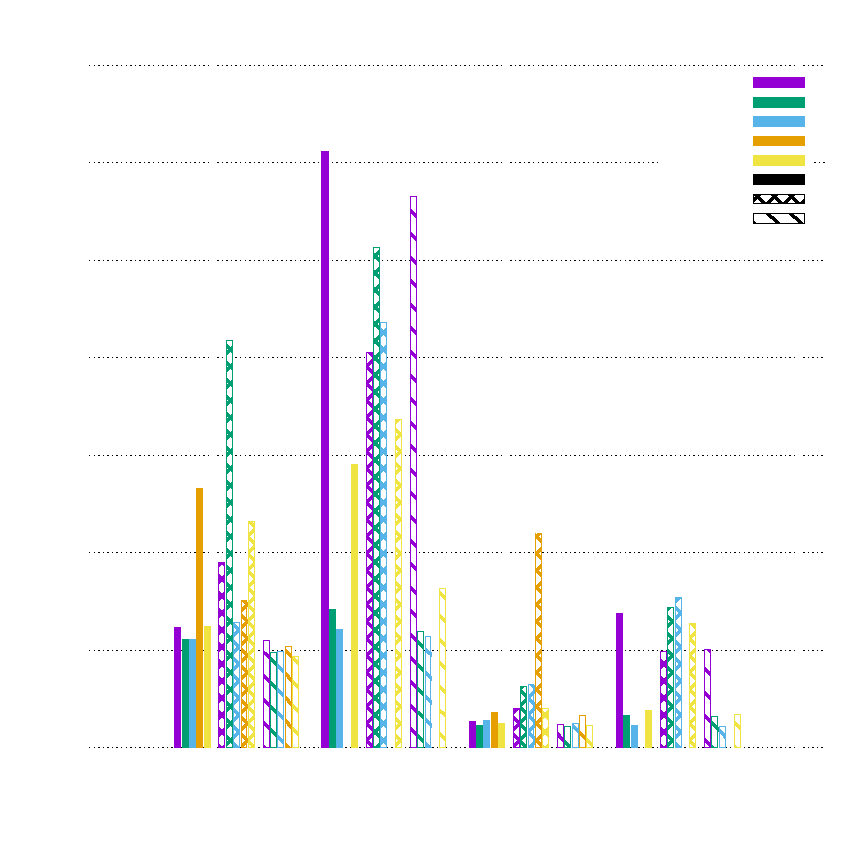
\includegraphics{desc_dist}}%
    \gplfronttext
  \end{picture}%
\endgroup

  \caption[Euclidean error scores per descriptors]{Euclidean error scores (sum of Euclidean distances for corresponding points) across the datasets for different descriptor algorithms. Similarly to Figure~\ref{fig:plot:euc_dist} the first two scores are for the initial estimates, using the reciprocal matching algorithm and the \gls{SAC-IA} respectively, the last score is for the final refining with \gls{ICP}, using initial estimate from the reciprocal matching algorithm. The reciprocal matching algorithm uses its default configuration of $k=5$ neighbours considered for matching.}
  \label{fig:plot:desc_dist}
\end{figure}

\section{Runtime performance}
\label{sec:runtime-perf}

Although the runtime performance was not a primary concern of the presented algorithm, it is interesting to take a look at the processing time. In the default configuration (Figure~\ref{fig:plot:perf}), there are orders of magnitude differences between algorithm steps as presented in Section~\ref{sec:estimate-pair-wise}. Most of the processing time is taken by the \gls{SIFT} keypoints detection and computation of \gls{PFH} descriptors.

\begin{figure}
  \centering
  % GNUPLOT: LaTeX picture with Postscript
\begingroup
  \makeatletter
  \providecommand\color[2][]{%
    \GenericError{(gnuplot) \space\space\space\@spaces}{%
      Package color not loaded in conjunction with
      terminal option `colourtext'%
    }{See the gnuplot documentation for explanation.%
    }{Either use 'blacktext' in gnuplot or load the package
      color.sty in LaTeX.}%
    \renewcommand\color[2][]{}%
  }%
  \providecommand\includegraphics[2][]{%
    \GenericError{(gnuplot) \space\space\space\@spaces}{%
      Package graphicx or graphics not loaded%
    }{See the gnuplot documentation for explanation.%
    }{The gnuplot epslatex terminal needs graphicx.sty or graphics.sty.}%
    \renewcommand\includegraphics[2][]{}%
  }%
  \providecommand\rotatebox[2]{#2}%
  \@ifundefined{ifGPcolor}{%
    \newif\ifGPcolor
    \GPcolortrue
  }{}%
  \@ifundefined{ifGPblacktext}{%
    \newif\ifGPblacktext
    \GPblacktextfalse
  }{}%
  % define a \g@addto@macro without @ in the name:
  \let\gplgaddtomacro\g@addto@macro
  % define empty templates for all commands taking text:
  \gdef\gplbacktext{}%
  \gdef\gplfronttext{}%
  \makeatother
  \ifGPblacktext
    % no textcolor at all
    \def\colorrgb#1{}%
    \def\colorgray#1{}%
  \else
    % gray or color?
    \ifGPcolor
      \def\colorrgb#1{\color[rgb]{#1}}%
      \def\colorgray#1{\color[gray]{#1}}%
      \expandafter\def\csname LTw\endcsname{\color{white}}%
      \expandafter\def\csname LTb\endcsname{\color{black}}%
      \expandafter\def\csname LTa\endcsname{\color{black}}%
      \expandafter\def\csname LT0\endcsname{\color[rgb]{1,0,0}}%
      \expandafter\def\csname LT1\endcsname{\color[rgb]{0,1,0}}%
      \expandafter\def\csname LT2\endcsname{\color[rgb]{0,0,1}}%
      \expandafter\def\csname LT3\endcsname{\color[rgb]{1,0,1}}%
      \expandafter\def\csname LT4\endcsname{\color[rgb]{0,1,1}}%
      \expandafter\def\csname LT5\endcsname{\color[rgb]{1,1,0}}%
      \expandafter\def\csname LT6\endcsname{\color[rgb]{0,0,0}}%
      \expandafter\def\csname LT7\endcsname{\color[rgb]{1,0.3,0}}%
      \expandafter\def\csname LT8\endcsname{\color[rgb]{0.5,0.5,0.5}}%
    \else
      % gray
      \def\colorrgb#1{\color{black}}%
      \def\colorgray#1{\color[gray]{#1}}%
      \expandafter\def\csname LTw\endcsname{\color{white}}%
      \expandafter\def\csname LTb\endcsname{\color{black}}%
      \expandafter\def\csname LTa\endcsname{\color{black}}%
      \expandafter\def\csname LT0\endcsname{\color{black}}%
      \expandafter\def\csname LT1\endcsname{\color{black}}%
      \expandafter\def\csname LT2\endcsname{\color{black}}%
      \expandafter\def\csname LT3\endcsname{\color{black}}%
      \expandafter\def\csname LT4\endcsname{\color{black}}%
      \expandafter\def\csname LT5\endcsname{\color{black}}%
      \expandafter\def\csname LT6\endcsname{\color{black}}%
      \expandafter\def\csname LT7\endcsname{\color{black}}%
      \expandafter\def\csname LT8\endcsname{\color{black}}%
    \fi
  \fi
    \setlength{\unitlength}{0.0500bp}%
    \ifx\gptboxheight\undefined%
      \newlength{\gptboxheight}%
      \newlength{\gptboxwidth}%
      \newsavebox{\gptboxtext}%
    \fi%
    \setlength{\fboxrule}{0.5pt}%
    \setlength{\fboxsep}{1pt}%
\begin{picture}(8220.00,8220.00)%
    \gplgaddtomacro\gplbacktext{%
      \csname LTb\endcsname%%
      \put(849,1051){\makebox(0,0)[r]{\strut{}$0$}}%
      \csname LTb\endcsname%%
      \put(849,1870){\makebox(0,0)[r]{\strut{}$10000$}}%
      \csname LTb\endcsname%%
      \put(849,2688){\makebox(0,0)[r]{\strut{}$20000$}}%
      \csname LTb\endcsname%%
      \put(849,3507){\makebox(0,0)[r]{\strut{}$30000$}}%
      \csname LTb\endcsname%%
      \put(849,4325){\makebox(0,0)[r]{\strut{}$40000$}}%
      \csname LTb\endcsname%%
      \put(849,5144){\makebox(0,0)[r]{\strut{}$50000$}}%
      \csname LTb\endcsname%%
      \put(849,5962){\makebox(0,0)[r]{\strut{}$60000$}}%
      \csname LTb\endcsname%%
      \put(849,6781){\makebox(0,0)[r]{\strut{}$70000$}}%
      \csname LTb\endcsname%%
      \put(849,7599){\makebox(0,0)[r]{\strut{}$80000$}}%
      \csname LTb\endcsname%%
      \put(2343,949){\rotatebox{-45}{\makebox(0,0)[l]{\strut{}AAU forest}}}%
      \csname LTb\endcsname%%
      \put(3736,949){\rotatebox{-45}{\makebox(0,0)[l]{\strut{}Machine Hall}}}%
      \csname LTb\endcsname%%
      \put(5128,949){\rotatebox{-45}{\makebox(0,0)[l]{\strut{}Vicon Room 1}}}%
      \csname LTb\endcsname%%
      \put(6521,949){\rotatebox{-45}{\makebox(0,0)[l]{\strut{}Vicon Room 2}}}%
    }%
    \gplgaddtomacro\gplfronttext{%
      \csname LTb\endcsname%%
      \put(153,4325){\rotatebox{-270}{\makebox(0,0){\strut{}Time (ms)}}}%
      \csname LTb\endcsname%%
      \put(4432,7940){\makebox(0,0){\strut{}Performace}}%
      \csname LTb\endcsname%%
      \put(3399,7432){\makebox(0,0)[r]{\strut{}downsampling}}%
      \csname LTb\endcsname%%
      \put(3399,7246){\makebox(0,0)[r]{\strut{}removing outliers}}%
      \csname LTb\endcsname%%
      \put(3399,7060){\makebox(0,0)[r]{\strut{}normals computation}}%
      \csname LTb\endcsname%%
      \put(3399,6874){\makebox(0,0)[r]{\strut{}keypoints detection}}%
      \csname LTb\endcsname%%
      \put(3399,6688){\makebox(0,0)[r]{\strut{}descriptors computation}}%
      \csname LTb\endcsname%%
      \put(3399,6502){\makebox(0,0)[r]{\strut{}finding correspondences}}%
      \csname LTb\endcsname%%
      \put(3399,6316){\makebox(0,0)[r]{\strut{}ICP alignment}}%
    }%
    \gplbacktext
    \put(0,0){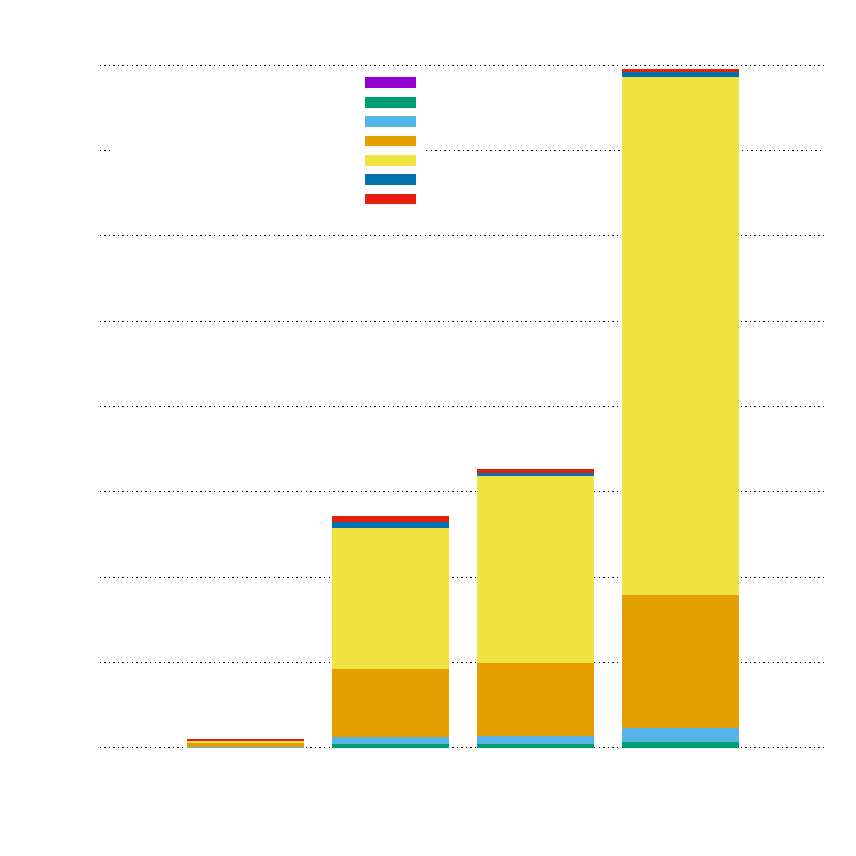
\includegraphics{perf}}%
    \gplfronttext
  \end{picture}%
\endgroup

  \caption[Processing time per algorithm parts]{Processing time for the respective parts of the map-merging algorithm (Section~\ref{sec:estimate-pair-wise}) across the datasets. The data has been recorded during one run of the algorithm on Intel(R) Core(TM) i5-2520M and do not incorporate measurements from multiple runs to deal with various sources of non-determinism, although the runtime of the algorithm has been observed to be quite stable. The data are intended to show order of magnitude differences of processing time between particular parts of the algorithm. The map-merging algorithm has been run with default parameters including \gls{PFH} descriptors and \gls{SIFT} keypoints.}
  \label{fig:plot:perf}
\end{figure}

There are, however, significant differences between descriptors regarding processing time (Figure~\ref{fig:plot:desc_perf}). All \gls{PFH}-family descriptors require orders of magnitude higher processing time. There are also significant differences between the \gls{PFH}-family, the processing time nearly doubles between \gls{FPFH}, \gls{PFH} and \gls{PFHRGB} descriptors.

The \gls{SHOT} descriptors with colour are very fast, which makes them a compelling choice, considering also they showed good robustness (Figure~\ref{fig:plot:desc_inliers}). \gls{PFHRGB} descriptors exhibited the best robustness, but also the longest processing time.

\begin{figure}
  \centering
  % GNUPLOT: LaTeX picture with Postscript
\begingroup
  \makeatletter
  \providecommand\color[2][]{%
    \GenericError{(gnuplot) \space\space\space\@spaces}{%
      Package color not loaded in conjunction with
      terminal option `colourtext'%
    }{See the gnuplot documentation for explanation.%
    }{Either use 'blacktext' in gnuplot or load the package
      color.sty in LaTeX.}%
    \renewcommand\color[2][]{}%
  }%
  \providecommand\includegraphics[2][]{%
    \GenericError{(gnuplot) \space\space\space\@spaces}{%
      Package graphicx or graphics not loaded%
    }{See the gnuplot documentation for explanation.%
    }{The gnuplot epslatex terminal needs graphicx.sty or graphics.sty.}%
    \renewcommand\includegraphics[2][]{}%
  }%
  \providecommand\rotatebox[2]{#2}%
  \@ifundefined{ifGPcolor}{%
    \newif\ifGPcolor
    \GPcolortrue
  }{}%
  \@ifundefined{ifGPblacktext}{%
    \newif\ifGPblacktext
    \GPblacktextfalse
  }{}%
  % define a \g@addto@macro without @ in the name:
  \let\gplgaddtomacro\g@addto@macro
  % define empty templates for all commands taking text:
  \gdef\gplbacktext{}%
  \gdef\gplfronttext{}%
  \makeatother
  \ifGPblacktext
    % no textcolor at all
    \def\colorrgb#1{}%
    \def\colorgray#1{}%
  \else
    % gray or color?
    \ifGPcolor
      \def\colorrgb#1{\color[rgb]{#1}}%
      \def\colorgray#1{\color[gray]{#1}}%
      \expandafter\def\csname LTw\endcsname{\color{white}}%
      \expandafter\def\csname LTb\endcsname{\color{black}}%
      \expandafter\def\csname LTa\endcsname{\color{black}}%
      \expandafter\def\csname LT0\endcsname{\color[rgb]{1,0,0}}%
      \expandafter\def\csname LT1\endcsname{\color[rgb]{0,1,0}}%
      \expandafter\def\csname LT2\endcsname{\color[rgb]{0,0,1}}%
      \expandafter\def\csname LT3\endcsname{\color[rgb]{1,0,1}}%
      \expandafter\def\csname LT4\endcsname{\color[rgb]{0,1,1}}%
      \expandafter\def\csname LT5\endcsname{\color[rgb]{1,1,0}}%
      \expandafter\def\csname LT6\endcsname{\color[rgb]{0,0,0}}%
      \expandafter\def\csname LT7\endcsname{\color[rgb]{1,0.3,0}}%
      \expandafter\def\csname LT8\endcsname{\color[rgb]{0.5,0.5,0.5}}%
    \else
      % gray
      \def\colorrgb#1{\color{black}}%
      \def\colorgray#1{\color[gray]{#1}}%
      \expandafter\def\csname LTw\endcsname{\color{white}}%
      \expandafter\def\csname LTb\endcsname{\color{black}}%
      \expandafter\def\csname LTa\endcsname{\color{black}}%
      \expandafter\def\csname LT0\endcsname{\color{black}}%
      \expandafter\def\csname LT1\endcsname{\color{black}}%
      \expandafter\def\csname LT2\endcsname{\color{black}}%
      \expandafter\def\csname LT3\endcsname{\color{black}}%
      \expandafter\def\csname LT4\endcsname{\color{black}}%
      \expandafter\def\csname LT5\endcsname{\color{black}}%
      \expandafter\def\csname LT6\endcsname{\color{black}}%
      \expandafter\def\csname LT7\endcsname{\color{black}}%
      \expandafter\def\csname LT8\endcsname{\color{black}}%
    \fi
  \fi
    \setlength{\unitlength}{0.0500bp}%
    \ifx\gptboxheight\undefined%
      \newlength{\gptboxheight}%
      \newlength{\gptboxwidth}%
      \newsavebox{\gptboxtext}%
    \fi%
    \setlength{\fboxrule}{0.5pt}%
    \setlength{\fboxsep}{1pt}%
\begin{picture}(8220.00,8220.00)%
    \gplgaddtomacro\gplbacktext{%
      \csname LTb\endcsname%%
      \put(951,1051){\makebox(0,0)[r]{\strut{}$0$}}%
      \csname LTb\endcsname%%
      \put(951,2142){\makebox(0,0)[r]{\strut{}$20000$}}%
      \csname LTb\endcsname%%
      \put(951,3234){\makebox(0,0)[r]{\strut{}$40000$}}%
      \csname LTb\endcsname%%
      \put(951,4325){\makebox(0,0)[r]{\strut{}$60000$}}%
      \csname LTb\endcsname%%
      \put(951,5416){\makebox(0,0)[r]{\strut{}$80000$}}%
      \csname LTb\endcsname%%
      \put(951,6508){\makebox(0,0)[r]{\strut{}$100000$}}%
      \csname LTb\endcsname%%
      \put(951,7599){\makebox(0,0)[r]{\strut{}$120000$}}%
      \csname LTb\endcsname%%
      \put(2425,949){\rotatebox{-45}{\makebox(0,0)[l]{\strut{}AAU forest}}}%
      \csname LTb\endcsname%%
      \put(3797,949){\rotatebox{-45}{\makebox(0,0)[l]{\strut{}Machine Hall}}}%
      \csname LTb\endcsname%%
      \put(5169,949){\rotatebox{-45}{\makebox(0,0)[l]{\strut{}Vicon Room 1}}}%
      \csname LTb\endcsname%%
      \put(6541,949){\rotatebox{-45}{\makebox(0,0)[l]{\strut{}Vicon Room 2}}}%
    }%
    \gplgaddtomacro\gplfronttext{%
      \csname LTb\endcsname%%
      \put(153,4325){\rotatebox{-270}{\makebox(0,0){\strut{}Time (ms)}}}%
      \csname LTb\endcsname%%
      \put(4483,7940){\makebox(0,0){\strut{}Computation time for descriptors}}%
      \csname LTb\endcsname%%
      \put(1767,7432){\makebox(0,0)[r]{\strut{}FPFH}}%
      \csname LTb\endcsname%%
      \put(1767,7246){\makebox(0,0)[r]{\strut{}PFH}}%
      \csname LTb\endcsname%%
      \put(1767,7060){\makebox(0,0)[r]{\strut{}PFHRGB}}%
      \csname LTb\endcsname%%
      \put(1767,6874){\makebox(0,0)[r]{\strut{}SC3D}}%
      \csname LTb\endcsname%%
      \put(1767,6688){\makebox(0,0)[r]{\strut{}SHOT}}%
    }%
    \gplbacktext
    \put(0,0){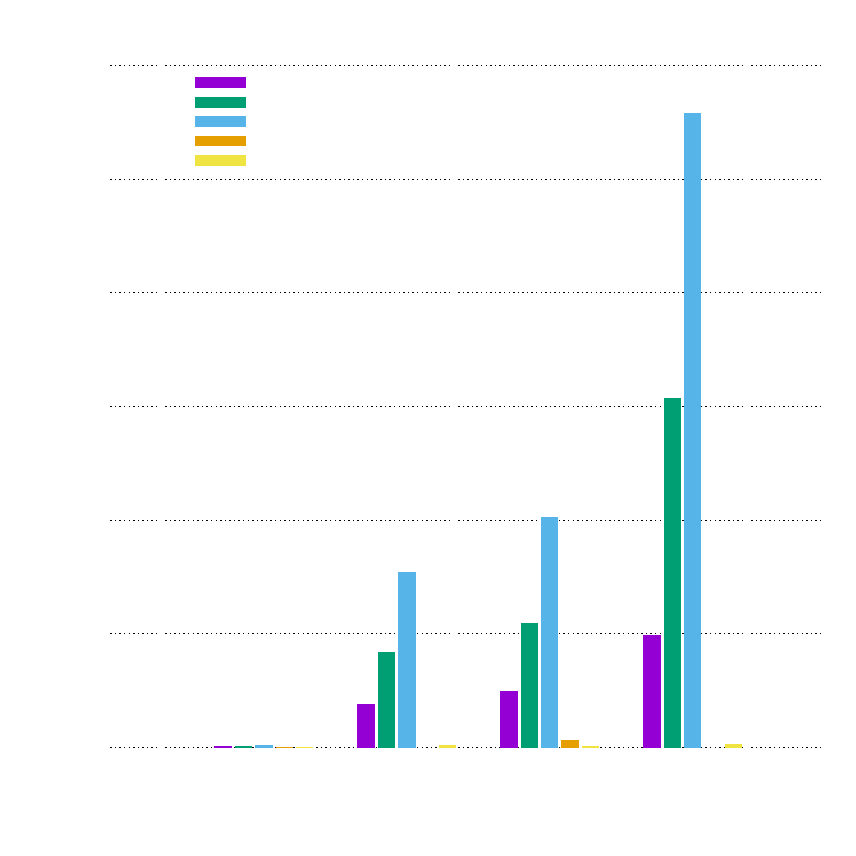
\includegraphics{desc_perf}}%
    \gplfronttext
  \end{picture}%
\endgroup

  \caption[Processing time per descriptors]{Processing time for descriptors algorithms across the datasets. Similarly to Figure~\ref{fig:plot:perf}, the data has been recorded during one run of the algorithm on Intel(R) Core(TM) i5-2520M and are intended to show order of magnitude differences of processing time between particular descriptors.}
  \label{fig:plot:desc_perf}
\end{figure}

\section{Initial estimate algorithms}
\label{sec:initial-estimate-algorithms}

Comparing the presented reciprocal matching algorithm (Algorithm~\ref{alg:cross-match}) with \gls{SAC-IA}, the reciprocal matching algorithm produces a better initial estimate in most of the evaluated cases (Figure~\ref{fig:plot:desc_dist}). A significantly worse initial estimate was produced only for the \gls{FPFH} descriptors in ``Machine Hall'' dataset, which may not come as a surprise as the \gls{SAC-IA} algorithm was introduced with \gls{FPFH} descriptors.

For \gls{PFH}, \gls{PFHRGB} and \gls{SHOT} descriptors the reciprocal matching algorithm produced better initial estimates in the evaluation than the \gls{SAC-IA} algorithm. Especially for the \gls{PFH} and \gls{PFHRGB} descriptors, the Euclidean error distance is significantly lower for the initial estimates produced by the reciprocal matching algorithm.

\begin{figure}
  \centering
  % GNUPLOT: LaTeX picture with Postscript
\begingroup
  \makeatletter
  \providecommand\color[2][]{%
    \GenericError{(gnuplot) \space\space\space\@spaces}{%
      Package color not loaded in conjunction with
      terminal option `colourtext'%
    }{See the gnuplot documentation for explanation.%
    }{Either use 'blacktext' in gnuplot or load the package
      color.sty in LaTeX.}%
    \renewcommand\color[2][]{}%
  }%
  \providecommand\includegraphics[2][]{%
    \GenericError{(gnuplot) \space\space\space\@spaces}{%
      Package graphicx or graphics not loaded%
    }{See the gnuplot documentation for explanation.%
    }{The gnuplot epslatex terminal needs graphicx.sty or graphics.sty.}%
    \renewcommand\includegraphics[2][]{}%
  }%
  \providecommand\rotatebox[2]{#2}%
  \@ifundefined{ifGPcolor}{%
    \newif\ifGPcolor
    \GPcolortrue
  }{}%
  \@ifundefined{ifGPblacktext}{%
    \newif\ifGPblacktext
    \GPblacktextfalse
  }{}%
  % define a \g@addto@macro without @ in the name:
  \let\gplgaddtomacro\g@addto@macro
  % define empty templates for all commands taking text:
  \gdef\gplbacktext{}%
  \gdef\gplfronttext{}%
  \makeatother
  \ifGPblacktext
    % no textcolor at all
    \def\colorrgb#1{}%
    \def\colorgray#1{}%
  \else
    % gray or color?
    \ifGPcolor
      \def\colorrgb#1{\color[rgb]{#1}}%
      \def\colorgray#1{\color[gray]{#1}}%
      \expandafter\def\csname LTw\endcsname{\color{white}}%
      \expandafter\def\csname LTb\endcsname{\color{black}}%
      \expandafter\def\csname LTa\endcsname{\color{black}}%
      \expandafter\def\csname LT0\endcsname{\color[rgb]{1,0,0}}%
      \expandafter\def\csname LT1\endcsname{\color[rgb]{0,1,0}}%
      \expandafter\def\csname LT2\endcsname{\color[rgb]{0,0,1}}%
      \expandafter\def\csname LT3\endcsname{\color[rgb]{1,0,1}}%
      \expandafter\def\csname LT4\endcsname{\color[rgb]{0,1,1}}%
      \expandafter\def\csname LT5\endcsname{\color[rgb]{1,1,0}}%
      \expandafter\def\csname LT6\endcsname{\color[rgb]{0,0,0}}%
      \expandafter\def\csname LT7\endcsname{\color[rgb]{1,0.3,0}}%
      \expandafter\def\csname LT8\endcsname{\color[rgb]{0.5,0.5,0.5}}%
    \else
      % gray
      \def\colorrgb#1{\color{black}}%
      \def\colorgray#1{\color[gray]{#1}}%
      \expandafter\def\csname LTw\endcsname{\color{white}}%
      \expandafter\def\csname LTb\endcsname{\color{black}}%
      \expandafter\def\csname LTa\endcsname{\color{black}}%
      \expandafter\def\csname LT0\endcsname{\color{black}}%
      \expandafter\def\csname LT1\endcsname{\color{black}}%
      \expandafter\def\csname LT2\endcsname{\color{black}}%
      \expandafter\def\csname LT3\endcsname{\color{black}}%
      \expandafter\def\csname LT4\endcsname{\color{black}}%
      \expandafter\def\csname LT5\endcsname{\color{black}}%
      \expandafter\def\csname LT6\endcsname{\color{black}}%
      \expandafter\def\csname LT7\endcsname{\color{black}}%
      \expandafter\def\csname LT8\endcsname{\color{black}}%
    \fi
  \fi
    \setlength{\unitlength}{0.0500bp}%
    \ifx\gptboxheight\undefined%
      \newlength{\gptboxheight}%
      \newlength{\gptboxwidth}%
      \newsavebox{\gptboxtext}%
    \fi%
    \setlength{\fboxrule}{0.5pt}%
    \setlength{\fboxsep}{1pt}%
\begin{picture}(8220.00,8220.00)%
    \gplgaddtomacro\gplbacktext{%
      \csname LTb\endcsname%%
      \put(357,1051){\makebox(0,0)[r]{\strut{}$0$}}%
      \csname LTb\endcsname%%
      \put(357,1779){\makebox(0,0)[r]{\strut{}$5$}}%
      \csname LTb\endcsname%%
      \put(357,2506){\makebox(0,0)[r]{\strut{}$10$}}%
      \csname LTb\endcsname%%
      \put(357,3234){\makebox(0,0)[r]{\strut{}$15$}}%
      \csname LTb\endcsname%%
      \put(357,3961){\makebox(0,0)[r]{\strut{}$20$}}%
      \csname LTb\endcsname%%
      \put(357,4689){\makebox(0,0)[r]{\strut{}$25$}}%
      \csname LTb\endcsname%%
      \put(357,5416){\makebox(0,0)[r]{\strut{}$30$}}%
      \csname LTb\endcsname%%
      \put(357,6144){\makebox(0,0)[r]{\strut{}$35$}}%
      \csname LTb\endcsname%%
      \put(357,6871){\makebox(0,0)[r]{\strut{}$40$}}%
      \csname LTb\endcsname%%
      \put(357,7599){\makebox(0,0)[r]{\strut{}$45$}}%
      \csname LTb\endcsname%%
      \put(1950,949){\rotatebox{-45}{\makebox(0,0)[l]{\strut{}AAU forest}}}%
      \csname LTb\endcsname%%
      \put(3441,949){\rotatebox{-45}{\makebox(0,0)[l]{\strut{}Machine Hall}}}%
      \csname LTb\endcsname%%
      \put(4931,949){\rotatebox{-45}{\makebox(0,0)[l]{\strut{}Vicon Room 1}}}%
      \csname LTb\endcsname%%
      \put(6422,949){\rotatebox{-45}{\makebox(0,0)[l]{\strut{}Vicon Room 2}}}%
    }%
    \gplgaddtomacro\gplfronttext{%
      \csname LTb\endcsname%%
      \put(4186,7940){\makebox(0,0){\strut{}Number of inliers for different matching strategies}}%
      \csname LTb\endcsname%%
      \put(1173,7432){\makebox(0,0)[r]{\strut{}FPFH}}%
      \csname LTb\endcsname%%
      \put(1173,7246){\makebox(0,0)[r]{\strut{}PFH}}%
      \csname LTb\endcsname%%
      \put(1173,7060){\makebox(0,0)[r]{\strut{}PFHRGB}}%
      \csname LTb\endcsname%%
      \put(1173,6874){\makebox(0,0)[r]{\strut{}SC3D}}%
      \csname LTb\endcsname%%
      \put(1173,6688){\makebox(0,0)[r]{\strut{}SHOT}}%
      \csname LTb\endcsname%%
      \put(1173,6502){\makebox(0,0)[r]{\strut{}k = 1}}%
      \csname LTb\endcsname%%
      \put(1173,6316){\makebox(0,0)[r]{\strut{}k = 5}}%
      \csname LTb\endcsname%%
      \put(1173,6130){\makebox(0,0)[r]{\strut{}k = 10}}%
    }%
    \gplbacktext
    \put(0,0){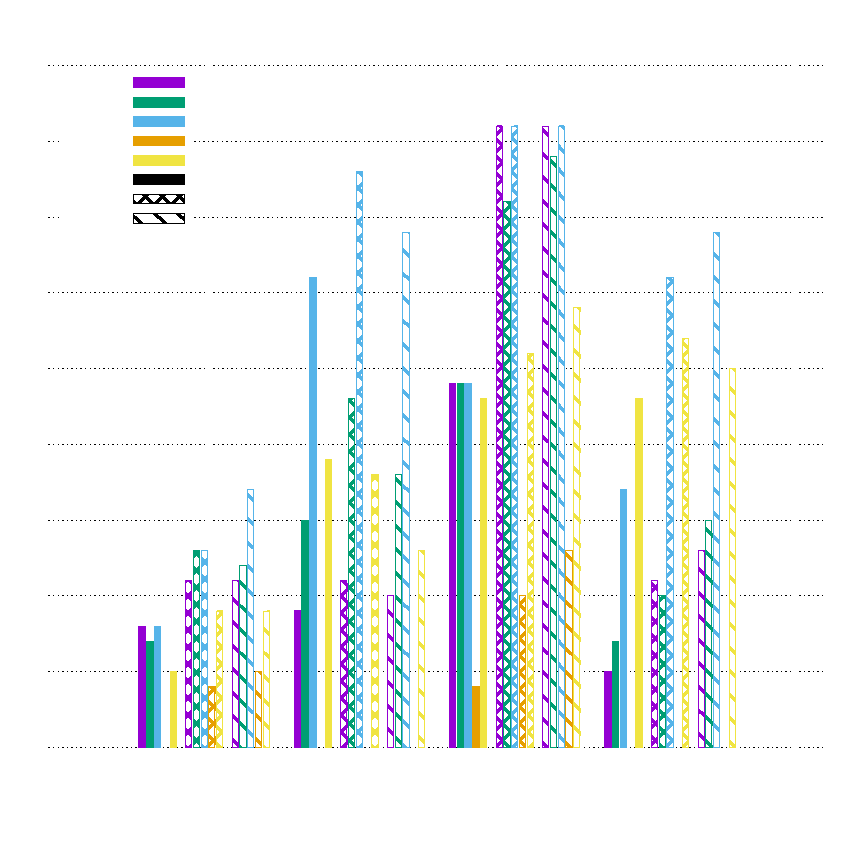
\includegraphics{matching_k_inliers}}%
    \gplfronttext
  \end{picture}%
\endgroup

  \caption[The number of inliers per $k$ in the reciprocal matching algorithm]{The number of inliers in matches produced by the presented reciprocal matching algorithm (Algorithm~\ref{alg:cross-match}) for different $k$ and the evaluated descriptors. For $k=1$ the algorithm is standard ``1-on-1'' matching with reciprocal match validation. The evaluation was running with default parameters.}
  \label{fig:plot:matching_k_inliers}
\end{figure}

\begin{figure}
  \centering
  % GNUPLOT: LaTeX picture with Postscript
\begingroup
  \makeatletter
  \providecommand\color[2][]{%
    \GenericError{(gnuplot) \space\space\space\@spaces}{%
      Package color not loaded in conjunction with
      terminal option `colourtext'%
    }{See the gnuplot documentation for explanation.%
    }{Either use 'blacktext' in gnuplot or load the package
      color.sty in LaTeX.}%
    \renewcommand\color[2][]{}%
  }%
  \providecommand\includegraphics[2][]{%
    \GenericError{(gnuplot) \space\space\space\@spaces}{%
      Package graphicx or graphics not loaded%
    }{See the gnuplot documentation for explanation.%
    }{The gnuplot epslatex terminal needs graphicx.sty or graphics.sty.}%
    \renewcommand\includegraphics[2][]{}%
  }%
  \providecommand\rotatebox[2]{#2}%
  \@ifundefined{ifGPcolor}{%
    \newif\ifGPcolor
    \GPcolortrue
  }{}%
  \@ifundefined{ifGPblacktext}{%
    \newif\ifGPblacktext
    \GPblacktextfalse
  }{}%
  % define a \g@addto@macro without @ in the name:
  \let\gplgaddtomacro\g@addto@macro
  % define empty templates for all commands taking text:
  \gdef\gplbacktext{}%
  \gdef\gplfronttext{}%
  \makeatother
  \ifGPblacktext
    % no textcolor at all
    \def\colorrgb#1{}%
    \def\colorgray#1{}%
  \else
    % gray or color?
    \ifGPcolor
      \def\colorrgb#1{\color[rgb]{#1}}%
      \def\colorgray#1{\color[gray]{#1}}%
      \expandafter\def\csname LTw\endcsname{\color{white}}%
      \expandafter\def\csname LTb\endcsname{\color{black}}%
      \expandafter\def\csname LTa\endcsname{\color{black}}%
      \expandafter\def\csname LT0\endcsname{\color[rgb]{1,0,0}}%
      \expandafter\def\csname LT1\endcsname{\color[rgb]{0,1,0}}%
      \expandafter\def\csname LT2\endcsname{\color[rgb]{0,0,1}}%
      \expandafter\def\csname LT3\endcsname{\color[rgb]{1,0,1}}%
      \expandafter\def\csname LT4\endcsname{\color[rgb]{0,1,1}}%
      \expandafter\def\csname LT5\endcsname{\color[rgb]{1,1,0}}%
      \expandafter\def\csname LT6\endcsname{\color[rgb]{0,0,0}}%
      \expandafter\def\csname LT7\endcsname{\color[rgb]{1,0.3,0}}%
      \expandafter\def\csname LT8\endcsname{\color[rgb]{0.5,0.5,0.5}}%
    \else
      % gray
      \def\colorrgb#1{\color{black}}%
      \def\colorgray#1{\color[gray]{#1}}%
      \expandafter\def\csname LTw\endcsname{\color{white}}%
      \expandafter\def\csname LTb\endcsname{\color{black}}%
      \expandafter\def\csname LTa\endcsname{\color{black}}%
      \expandafter\def\csname LT0\endcsname{\color{black}}%
      \expandafter\def\csname LT1\endcsname{\color{black}}%
      \expandafter\def\csname LT2\endcsname{\color{black}}%
      \expandafter\def\csname LT3\endcsname{\color{black}}%
      \expandafter\def\csname LT4\endcsname{\color{black}}%
      \expandafter\def\csname LT5\endcsname{\color{black}}%
      \expandafter\def\csname LT6\endcsname{\color{black}}%
      \expandafter\def\csname LT7\endcsname{\color{black}}%
      \expandafter\def\csname LT8\endcsname{\color{black}}%
    \fi
  \fi
    \setlength{\unitlength}{0.0500bp}%
    \ifx\gptboxheight\undefined%
      \newlength{\gptboxheight}%
      \newlength{\gptboxwidth}%
      \newsavebox{\gptboxtext}%
    \fi%
    \setlength{\fboxrule}{0.5pt}%
    \setlength{\fboxsep}{1pt}%
\begin{picture}(8220.00,8220.00)%
    \gplgaddtomacro\gplbacktext{%
      \csname LTb\endcsname%%
      \put(747,1051){\makebox(0,0)[r]{\strut{}$0$}}%
      \csname LTb\endcsname%%
      \put(747,1986){\makebox(0,0)[r]{\strut{}$0.05$}}%
      \csname LTb\endcsname%%
      \put(747,2922){\makebox(0,0)[r]{\strut{}$0.1$}}%
      \csname LTb\endcsname%%
      \put(747,3857){\makebox(0,0)[r]{\strut{}$0.15$}}%
      \csname LTb\endcsname%%
      \put(747,4793){\makebox(0,0)[r]{\strut{}$0.2$}}%
      \csname LTb\endcsname%%
      \put(747,5728){\makebox(0,0)[r]{\strut{}$0.25$}}%
      \csname LTb\endcsname%%
      \put(747,6664){\makebox(0,0)[r]{\strut{}$0.3$}}%
      \csname LTb\endcsname%%
      \put(747,7599){\makebox(0,0)[r]{\strut{}$0.35$}}%
      \csname LTb\endcsname%%
      \put(2262,949){\rotatebox{-45}{\makebox(0,0)[l]{\strut{}AAU forest}}}%
      \csname LTb\endcsname%%
      \put(3675,949){\rotatebox{-45}{\makebox(0,0)[l]{\strut{}Machine Hall}}}%
      \csname LTb\endcsname%%
      \put(5087,949){\rotatebox{-45}{\makebox(0,0)[l]{\strut{}Vicon Room 1}}}%
      \csname LTb\endcsname%%
      \put(6500,949){\rotatebox{-45}{\makebox(0,0)[l]{\strut{}Vicon Room 2}}}%
    }%
    \gplgaddtomacro\gplfronttext{%
      \csname LTb\endcsname%%
      \put(153,4325){\rotatebox{-270}{\makebox(0,0){\strut{}Distance (m)}}}%
      \csname LTb\endcsname%%
      \put(4381,7940){\makebox(0,0){\strut{}Euclidean error distance for different matching strategies}}%
      \csname LTb\endcsname%%
      \put(7125,7432){\makebox(0,0)[r]{\strut{}FPFH}}%
      \csname LTb\endcsname%%
      \put(7125,7246){\makebox(0,0)[r]{\strut{}PFH}}%
      \csname LTb\endcsname%%
      \put(7125,7060){\makebox(0,0)[r]{\strut{}PFHRGB}}%
      \csname LTb\endcsname%%
      \put(7125,6874){\makebox(0,0)[r]{\strut{}SC3D}}%
      \csname LTb\endcsname%%
      \put(7125,6688){\makebox(0,0)[r]{\strut{}SHOT}}%
      \csname LTb\endcsname%%
      \put(7125,6502){\makebox(0,0)[r]{\strut{}k = 1}}%
      \csname LTb\endcsname%%
      \put(7125,6316){\makebox(0,0)[r]{\strut{}k = 5}}%
      \csname LTb\endcsname%%
      \put(7125,6130){\makebox(0,0)[r]{\strut{}k = 10}}%
    }%
    \gplbacktext
    \put(0,0){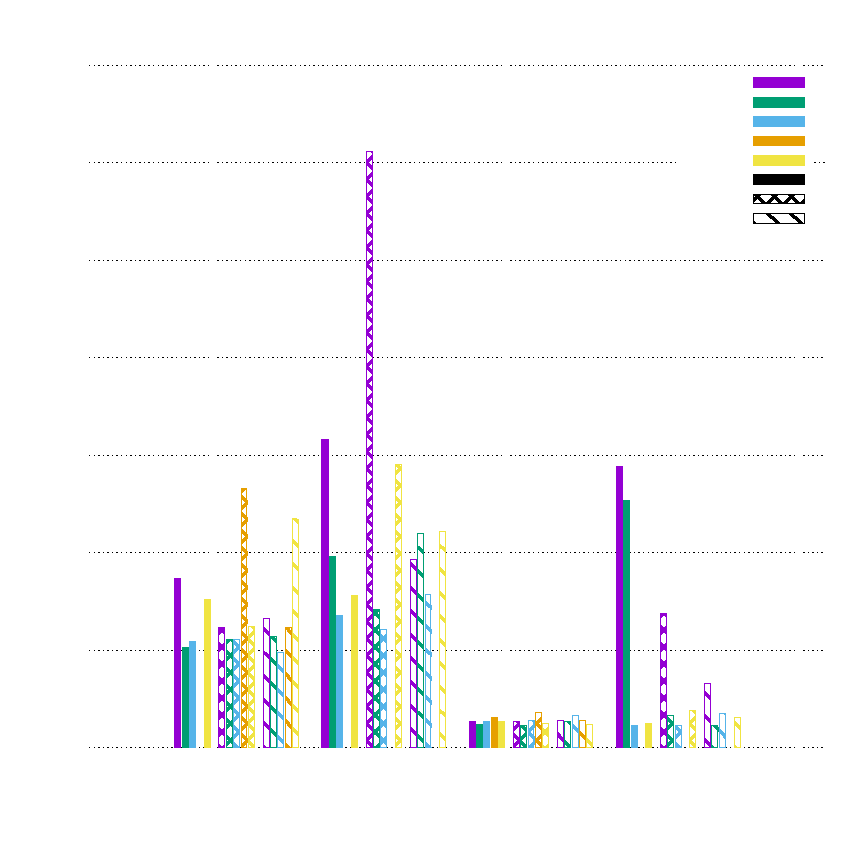
\includegraphics{matching_k_dist}}%
    \gplfronttext
  \end{picture}%
\endgroup

  \caption[The Euclidean distance per $k$ in the reciprocal matching algorithm]{The Euclidean error distance for different number of neighbours ($k$) of the presented reciprocal matching algorithm (Algorithm~\ref{alg:cross-match}). For $k=1$ the algorithm is standard ``1-on-1'' matching with reciprocal match validation. The evaluation was running with default parameters.}
  \label{fig:plot:matching_k_dist}
\end{figure}

Comparing the presented algorithm with standard ``1-on-1'' matching with reciprocal match validation, the presented approach can improve robustness in terms of number of inliers (Figure~\ref{fig:plot:matching_k_inliers}) and consecutively also accuracy in terms of smaller Euclidean distance (Figure~\ref{fig:plot:matching_k_dist}). The standard ``1-on-1'' matching, which considers only the nearest match, is equivalent to the presented reciprocal matching with $k=1$.

As expected, the increased number of neighbours considered for matching is beneficial for \gls{FPFH} descriptors, where increased $k$ is essential for a good initial estimate in some cases. With higher than default $k=10$, the reciprocal matching algorithm can produce a significantly better initial matching estimate than \gls{SAC-IA} algorithm.

Surprisingly, we can obverse the increased number of inliers also for \gls{PFH} and \gls{PFHRGB} descriptors with $k=5$ (Figure~\ref{fig:plot:matching_k_inliers}). Further broadening neighbour search to $k=10$ does not seem to increase robustness significantly for \gls{PFH} and \gls{PFHRGB} descriptors, in same cases the number of inliers is even lower than for $k=5$. The \gls{SHOT} descriptors with colour generally slightly benefit from increased $k$, but in the case of ``Machine Hall'' dataset the number of inliers decreases with increasing $k$. For \gls{SC3D} descriptors, there are less data as the implementation in \gls{PCL} crashed in ``Machine Hall'' and ``Vicon Room 2'' datasets. However it seems that \gls{SC3D} descriptors work well with the increased $k$, in ``AAU forest'' dataset there are no inliers for the standard ``1-on-1'' matching, but the presented matching approach was able to generate $5$ inliers with increased $k$, yielding a good initial estimate (Figure~\ref{fig:plot:matching_k_dist}).

Good performance across different descriptors makes the presented reciprocal matching a preferred matching strategy over \gls{SAC-IA} algorithm for the map-merging of point cloud maps.

\section{Overlapping areas}
\label{sec:mff-evaluation}

As the presented map-merging algorithm (Chapter~\ref{chap:mergingalgorithm}) relies entirely on information contained in the point cloud maps, properties of the overlapping area in maps (which is the only source of information for the map-merging) greatly influence the map-merging process.

First of all, the size of the common area in maps is the most influencing factor. Large common areas can possibly contain more features, which in turn can yield more feature matches and inliers providing a more robust transformation estimate.

In real-world environments, however, even a fairly large common areas might not be sufficient if they do not contain enough outstanding landmarks for the feature detection. These feature-poor areas are fairly common in man-made environments including industrial areas. Flat, single-colour surfaces typically pose a great challenge for common feature-based methods.

For example, ``MFF Refectory'' dataset (Figure~\ref{fig:mff_refectory}) contains two maps with an overlapping area at the corridor. Although the area is fairly large, it has proven to be insufficient for a reliable transformation estimate and the map-merging. The corridor does not contain enough significant landmarks. Moreover, the same lack of landmarks in corridor areas leads to mapping errors in the maps, that make map-merging even more challenging. If no common feature-rich areas are present in maps, the map-merging based exclusively on point cloud maps is expected to be a challenging task.

Ambiguities and self-similarities in the environment may also compromise the map-merging. ``MFF Rotunda'' dataset (Figure~\ref{fig:mff_rotunda}) was recorded in a symmetrical half-circular laboratory with many similarly looking workplaces. The symmetry of the environment causes \gls{SAC-IA} algorithm to wrongly match the maps upside down (Figure~\ref{fig:mff_rotunda_sac}).

\begin{figure}
    \centering
    \begin{subfigure}[b]{\textwidth}
        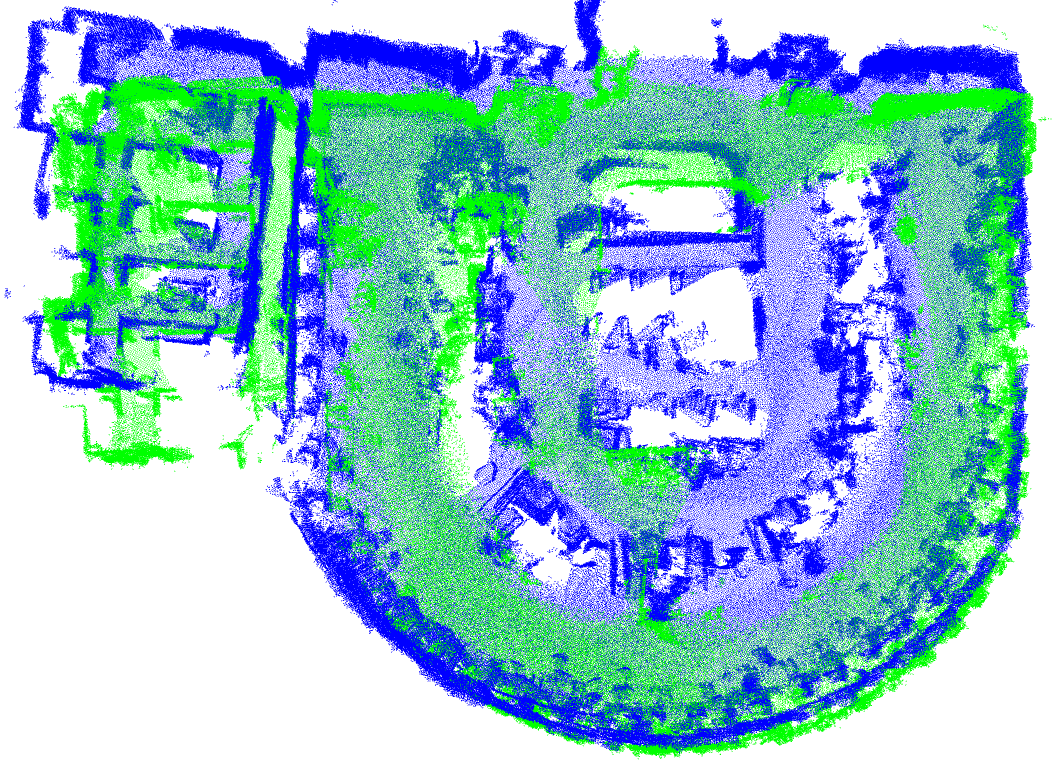
\includegraphics[width=\textwidth]{../img/mff_rotunda_sac_top.png}
        \caption{Top view}
    \end{subfigure}
    % ~
    \begin{subfigure}[b]{\textwidth}
        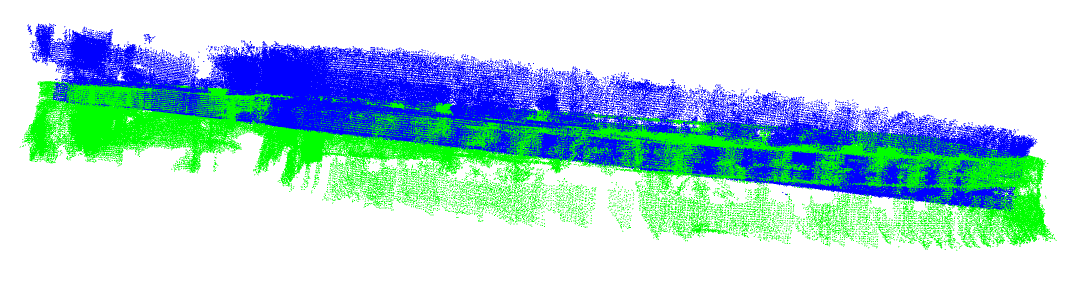
\includegraphics[width=\textwidth]{../img/mff_rotunda_sac_lateral.png}
        \caption{Lateral view}
    \end{subfigure}
    \caption[\gls{SAC-IA} initial estimate for ``MFF Rotunda '' dataset.]{The initial transformation estimate of \gls{SAC-IA} algorithm for ``MFF Rotunda'' dataset. The symmetry of the environment causes wrong upside down match of the second map.}
    \label{fig:mff_rotunda_sac}
\end{figure}

The presented reciprocal matching algorithm (Algorithm~\ref{alg:cross-match}) using a more strict non-probabilistic approach is able to avoid the upside down match. However, inliers are clustered in one particular area of the map (Figure~\ref{fig:mff_rotunda_matching_inliers}), which leads to a visible angular error (Figure~\ref{fig:mff_rotunda_matching_estimate}). Other parts of the common area proved unable to provide stable matches, especially the circular area seems to contain only unstable features and more mapping errors.

\begin{figure}
    \centering
    \begin{subfigure}[b]{\textwidth}
        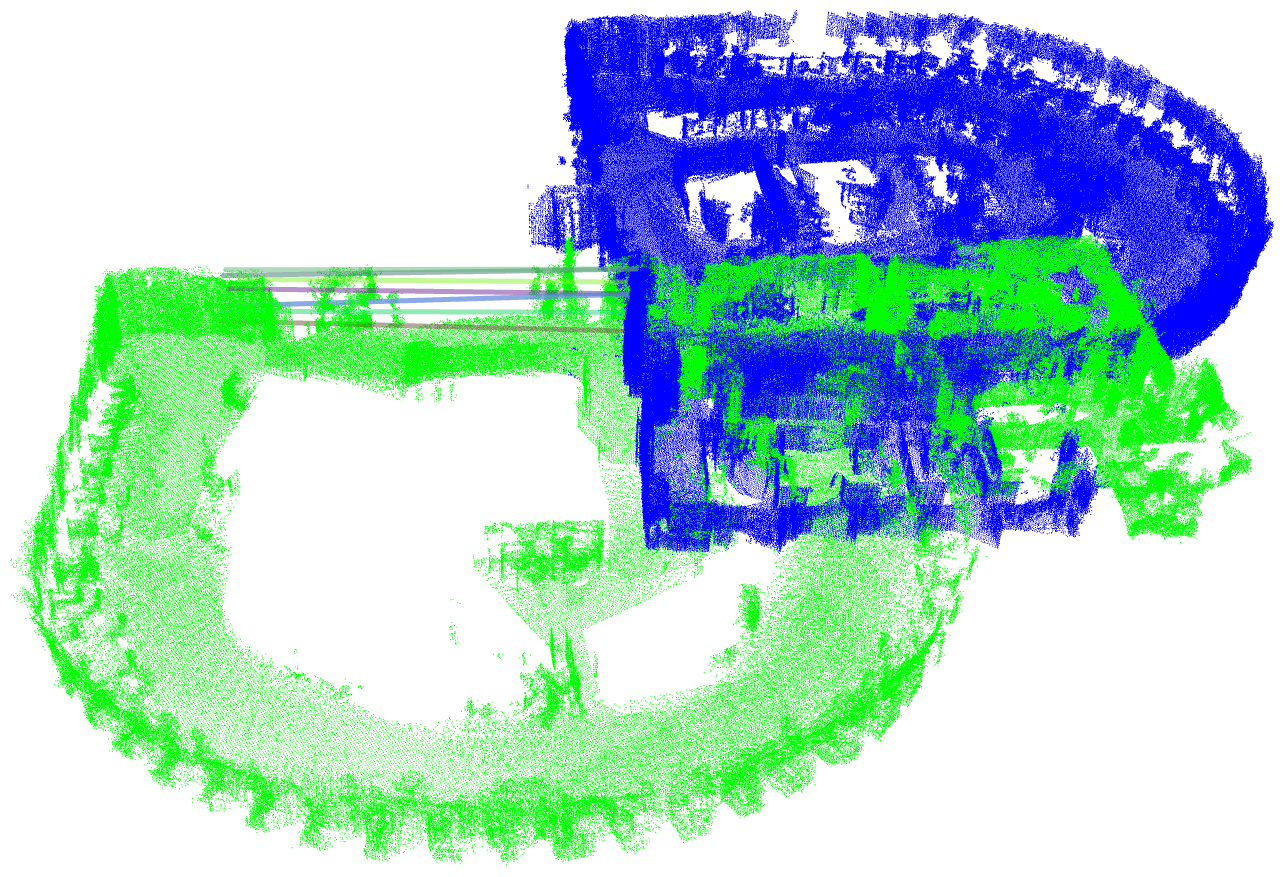
\includegraphics[width=\textwidth]{../img/mff_rotunda_matching_inliers.png}
        \caption{Inliers}
        \label{fig:mff_rotunda_matching_inliers}
    \end{subfigure}
    ~
    \begin{subfigure}[b]{\textwidth}
        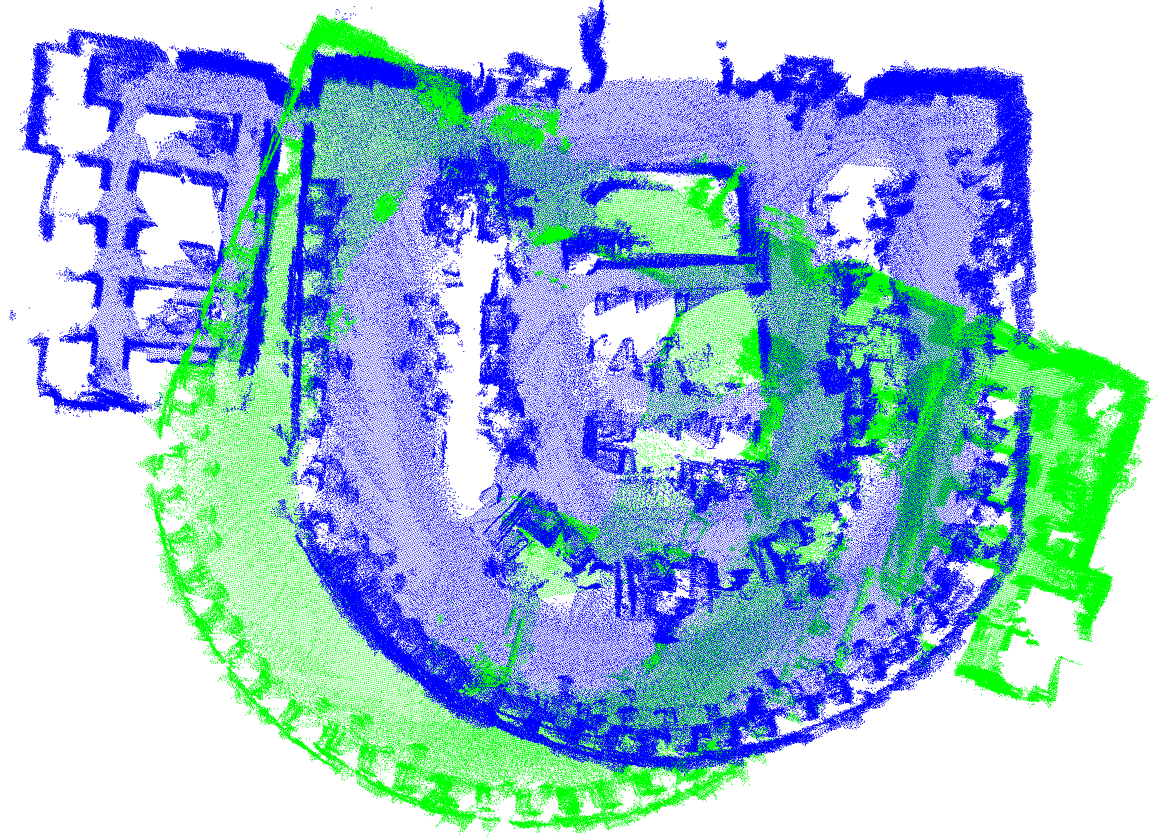
\includegraphics[width=\textwidth]{../img/mff_rotunda_matching_estimate.png}
        \caption{The initial estimate with an angular error}
        \label{fig:mff_rotunda_matching_estimate}
    \end{subfigure}
    \caption[The initial estimate for ``MFF Rotunda '' dataset produced by the reciprocal matching]{The initial transformation estimate and inliers of the presented reciprocal matching algorithm (Algorithm~\ref{alg:cross-match}) for ``MFF Rotunda'' dataset. The inliers are clustered in a single area, which introduces an angular error in the initial transformation estimate.}
    \label{fig:mff_rotunda_matching}
\end{figure}

This example shows that even fairly large common areas might not be suitable for the map-merging. Suitable common areas allowing a robust transformation estimate between maps should contain a decent amount of significant landmarks and should contain minimal amount of ambiguities, self-similarities and symmetries.
